\documentclass[a4paper, 11pt, spanish, twoside]{article}


%%%%%%%%%%%%%%%%% - PREÁMBULO - %%%%%%%%%%%%%%%%% 

% ------------------ Página -------------------- %
% Se define el tamaño de las páginas, indicando el tamaño de los márgenes superior e inferior ("top" y "bottom"), e izquierdo y derecho ("left" y "right"):
\usepackage[top=2.5cm,bottom=2.5cm,left=2.5cm,right=2.5cm]{geometry}
% Se inserta el comando \raggedbottom para evitar que LaTeX rellene con espacios en blanco aquellas páginas que no alberguen suficiente contenido como para rellenarlas de forma "natural":
\raggedbottom 
% ---------------------------------------------- %


% ------------- Paquetes generales ------------- %
% Se importan distintos paquetes de propósito general:
\usepackage[utf8]{inputenc}
\usepackage[spanish]{babel}
\usepackage{float}
\usepackage{caption}
% ---------------------------------------------- %


% ------------ Paquetes específicos ------------ %
% Se importan distintos paquetes que será utilizados en momentos concretos del documento: 
\usepackage{pdfpages} % Para insertar la portada en formato PDF.
\usepackage{amssymb} % Para símbolos matemáticos.
\usepackage{bm} % Para negrita en símbolos matemáticos.
\usepackage{amsmath} % Para el entorno "split".
\usepackage[hidelinks]{hyperref} % Para urls.
\usepackage{longtable} % Para tablas largas.
\usepackage{graphicx} % Para insertar imágenes.
\usepackage{wrapfig} % Para posicionar imágenes alrededor del texto.
\usepackage{fontawesome5} % Para utilizar iconos de "fontawesome".
\usepackage{pdflscape}  % Para colocar páginas en formato apaisado.
\usepackage[T1]{fontenc}
\usepackage{textcomp}
\usepackage{lmodern} % Soluciona el problema de la mala resolución
% ---------------------------------------------- %


% ---------------- Numeración ------------------ %
\counterwithin{table}{section} % Se numeran las tablas con respecto al capítulo en el que se encuentran.
\counterwithin{figure}{section} % Se numeran las figuras con respecto al capítulo en el que se encuentran.
\counterwithin{equation}{section} % Se numeran las ecuaciones con respecto al capítulo en el que se encuentran.
% ---------------------------------------------- %


% ------------- Página en blanco ----------------%
% Se define un comando (\blankpage) para insertar una página totalmente en blanco (sin número de página, encabezado y pie de página):
\usepackage{afterpage}
\newcommand\blankpage{%
    \null
    \thispagestyle{empty}%
    \newpage}
% ---------------------------------------------- %    


% ----------- Formato de los párrafos -----------%
% Se define el formato de los párrafos:
\setlength{\parindent}{0pt} % Se elimina la sangría en comienzo de párrafo (0pt).
\setlength{\parskip}{1em} % Se define el espacio entre dos párrafos (1em).
% ---------------------------------------------- %    

% -------------- Título adicional -------------- %
% Se añade una profundidad adicional a los títulos (profundidad 4):
\usepackage{titlesec}
\setcounter{secnumdepth}{4} % Se fija en 4 la profundidad de numeración de títulos.
\setcounter{tocdepth}{4} % Se fija en 4 la profundidad de títulos incluidos en el índice.
% Se modifica el formato de \paragraph (título de profundidad 4) para adaptarlo al formato del resto de títulos:
\titleformat{\paragraph}
{\normalfont\normalsize\bfseries}{\theparagraph}{1em}{}
\titlespacing*{\paragraph}
{0pt}{3.25ex plus 1ex minus .2ex}{1.5ex plus .2ex} 
% ---------------------------------------------- %    


% --------- Encabezado y pie de página -------- %
% El encabezado y pie de página forman parte del paquete fancyhdr:
\usepackage{fancyhdr}
\fancyhf{}
\pagestyle{fancy}

% Para solucionar error "headheight is too small":%
\setlength{\headheight}{14.6pt}
\addtolength{\topmargin}{-0.6pt}

% Se ajusta el tamaño de fuente para el encabezado y pie de página (9pt)
\fancyhf{\fontsize{2}{14}\selectfont}

% Contenido del encabezado (\fancyhead):
\fancyhead[RO]{Simulación de operación de una central nuclear} % Texto que se coloca en el encabezado de las páginas impares (O -> 'Odd', o impar) a la izquierda (R -> 'Odd')
\fancyhead[LE]{\nouppercase{\rightmark}} % Texto que se coloca en el encabezado de las páginas pares (E -> 'Even', o par) a la izquierda (L -> 'Left'). \rightmark se utiliza para insertar automáticamente el título de la sección correspondiente, y \nouppercase para que no aparezca todo en mayúsculas (formato por defecto de \rightmark).

% Contenido del pie de página (\fancyfoot):
\fancyfoot[RE]{Escuela  Técnica  Superior  de  Ingenieros  Industriales  (UPM)} % Texto que se coloca en el pie de página de las páginas pares (E -> 'Even', o par) a la derecha (R -> 'Right')
\fancyfoot[LO]{Antonio Dies Beneytez} % Texto que se coloca en el pie de página de las páginas impares (O -> 'Odd', o impar) a la izquierda (L -> 'Left')
\fancyfoot[LE,RO]{\thepage} % El número de página (\thepage) se coloca a la izquierda en las páginas pares y a la derecha en las impares.

% Se indica que sólo se quiere incorporar en \rightmark (utilizado más arriba) el título de la sección (y no de las subsecciones, subsubsecciones, etc.):
\renewcommand{\sectionmark}[1]{\markright{\thesection. #1}}
\renewcommand{\subsectionmark}[1]{}

% Formato de la línea de separación horizontal:
\renewcommand{\headrulewidth}{0.5pt} % Ancho de la línea del encabezado.
\renewcommand{\footrulewidth}{0.5pt} % Ancho de la línea del pie de página.
% ---------------------------------------------- % 


% ----------- Fragmentos de código ------------- %
% El paquete utilizado para insertar fragmentos de código en el documento es listings. En el presente bloque del preámbulo se definen ciertos parámetros de listings con el objetivo de adaptar dicho paquete a código escrito en Python.

\usepackage{listings} % Paquete para insertar código. 
\usepackage{xcolor} % Paquete para definir colores.

% Se definen los distintos colores que se utilizan para resaltar ciertos elementos del código:
\definecolor{codegreen}{rgb}{0.04314,0.6745,0.07843} % Verde.
\definecolor{codegray}{rgb}{0.5,0.5,0.5} % Gris.
\definecolor{codered}{rgb}{0.5373,0.02745,0.06275} % Rojo.
\definecolor{codeblue}{rgb}{0.071,0.0258,0.9882} % Azul.
\definecolor{codepurple}{rgb}{0.6,0.02745,0.5961} % Morado.

% Se define el color de fondo:
\definecolor{backcolour}{rgb}{0.95,0.95,0.92} % Gris oscuro.

% Se define el valor de ciertos parámetros de listings para adaptar dicho paquete a código escrito en Python:
\lstdefinestyle{mystyle}{
    % - General:
    language=Python, % Lenguaje de programación.
    basicstyle=\ttfamily\footnotesize, % Tipografía y tamaño de fuente.
    % - Colores de los distintos elementos del código:
    backgroundcolor=\color{backcolour}, % Color de fondo.  
    commentstyle=\color{codegray}, % Color de los comentarios.
    keywordstyle=\color{codeblue}, % Color de las palabras clave por defecto.
    stringstyle=\color{codegreen}, % Color de los "string"
    % - Palabras clave:
    deletekeywords={print}, % Se elimina "print" del conjunto de palabras clave para posteriormente asignarle el color morado.
    keywordstyle={[2]\ttfamily\color{codeblue}},
    keywords=[2]{as}, % Se añaden las palabras clave de color azul.
    keywordstyle={[3]\ttfamily\color{codepurple}},
    keywords=[3]{True, False, ttk, list, None, dict, zip, range, len, print, float, sum}, % Se añaden las palabras clave de color morado.
    keywordstyle={[4]\bfseries\ttfamily},
    keywords=[4]{_read_excel}, % Se añaden las palabras clave en negrita.
    emph={MyClass,__init__}, % Se añaden las palabras clave enfatizadas.   
    % - Números de línea:
    numberstyle=\tiny\color{codegray}, % Tamaño de fuente y color de los números de línea.
    numbers=left, % Se colocan los números de línea en el lado izquierdo.                 
    numbersep=5pt, % Separación horizontal de los números de línea.
    % - Saltos a la línea, espacios, indentación:
    breaklines=true, % Permitir saltos a la línea. 
    breakatwhitespace=true, % Saltar a la línea únicamente al encontrar espacios.
    postbreak = \mbox{{$\hookrightarrow$}\space}, % Se añade una flecha al cambiar de línea.
    showspaces=false, % No mostrar los espacios. 
    showstringspaces=false, % No mostrar los espacios en los "string".
    keepspaces=true, % Mantener los espacios presentes en el código. 
    tabsize=2, % Tamaño de indentación.
    % - Título:
    captionpos=b % Posición del título del fragmento de código (b=bottom - abajo).
} 
\lstset{style=mystyle} % Se asocia el estilo de listings al estilo que acaba de definirse ("mystyle")

% Se realizan una serie de operaciones complementarias con el paquete listings (su comprensión no es necesaria para manejar dicho paquete):
\makeatletter
\def\lst@OpLiteratekey#1\@nil@{\let\lst@ifxopliterate\lst@if
                             \def\lst@opliterate{#1}}
\lst@Key{opliterate}{}{\@ifstar{\lst@true \lst@OpLiteratekey}
                             {\lst@false\lst@OpLiteratekey}#1\@nil@}
\lst@AddToHook{SelectCharTable}
    {\ifx\lst@opliterate\@empty\else
         \expandafter\lst@OpLiterate\lst@opliterate{}\relax\z@
     \fi}
\def\lst@OpLiterate#1#2#3{%
    \ifx\relax#2\@empty\else
        \lst@CArgX #1\relax\lst@CDef
            {}
            {\let\lst@next\@empty
             \lst@ifxopliterate
                \lst@ifmode \let\lst@next\lst@CArgEmpty \fi
             \fi
             \ifx\lst@next\@empty
                 \ifx\lst@OutputBox\@gobble\else
                   \lst@XPrintToken \let\lst@scanmode\lst@scan@m
                   \lst@token{#2}\lst@length#3\relax
                   \lst@XPrintToken
                 \fi
                 \let\lst@next\lst@CArgEmptyGobble
             \fi
             \lst@next}%
            \@empty
        \expandafter\lst@OpLiterate
    \fi}

\lstset{ 
    literate={á}{{\'a}}1 {é}{{\'e}}1 {í}{{\'i}}1 {ó}{{\'o}}1 {ú}{{\'u}}1
  {Á}{{\'A}}1 {É}{{\'E}}1 {Í}{{\'I}}1 {Ó}{{\'O}}1 {Ú}{{\'U}}1
  {à}{{\`a}}1 {è}{{\`e}}1 {ì}{{\`i}}1 {ò}{{\`o}}1 {ù}{{\`u}}1
  {À}{{\`A}}1 {È}{{\'E}}1 {Ì}{{\`I}}1 {Ò}{{\`O}}1 {Ù}{{\`U}}1
  {ä}{{\"a}}1 {ë}{{\"e}}1 {ï}{{\"i}}1 {ö}{{\"o}}1 {ü}{{\"u}}1
  {Ä}{{\"A}}1 {Ë}{{\"E}}1 {Ï}{{\"I}}1 {Ö}{{\"O}}1 {Ü}{{\"U}}1
  {â}{{\^a}}1 {ê}{{\^e}}1 {î}{{\^i}}1 {ô}{{\^o}}1 {û}{{\^u}}1
  {Â}{{\^A}}1 {Ê}{{\^E}}1 {Î}{{\^I}}1 {Ô}{{\^O}}1 {Û}{{\^U}}1
  {Ã}{{\~A}}1 {ã}{{\~a}}1 {Õ}{{\~O}}1 {õ}{{\~o}}1
  {œ}{{\oe}}1 {Œ}{{\OE}}1 {æ}{{\ae}}1 {Æ}{{\AE}}1 {ß}{{\ss}}1
  {ű}{{\H{u}}}1 {Ű}{{\H{U}}}1 {ő}{{\H{o}}}1 {Ő}{{\H{O}}}1
  {ç}{{\c c}}1 {Ç}{{\c C}}1 {ø}{{\o}}1 {å}{{\r a}}1 {Å}{{\r A}}1
  {€}{{\euro}}1 {£}{{\pounds}}1 {«}{{\guillemotleft}}1
  {»}{{\guillemotright}}1 {ñ}{{\~n}}1 {Ñ}{{\~N}}1 {¿}{{?`}}1
  {º}{{\textordmasculine}}1}

\lstset{opliterate=
   *{0}{{{\color{codered}0}}}1 {1}{{{\color{codered}1}}}1 
   {2}{{{\color{codered}2}}}1 {3}{{{\color{codered}3}}}1 
   {4}{{{\color{codered}4}}}1 {5}{{{\color{codered}5}}}1 
   {6}{{{\color{codered}6}}}1 {7}{{{\color{codered}7}}}1 
   {8}{{{\color{codered}8}}}1 {9}{{{\color{codered}9}}}1}

\DeclareCaptionType{code}[Código][ÍNDICE DE CÓDIGOS] % Se define el entorno "Código" (de forma que al introducir un fragmento de código en el documento aparezca como: Código 1.1: ...), y la lista con los distintos códigos ("Índice de códigos").
\counterwithin{code}{section} % Se numeran los códigos con respecto al capítulo en el que se encuentran.
% ---------------------------------------------- % 


% --------------- Bibliografía ----------------- %
% El manejo de la bibliografía se realiza mediante el paquete biblatex:
\usepackage[backend=bibtex, style=authoryear, sorting=nyt, citestyle=authoryear, maxcitenames=2, maxbibnames=5, giveninits=true, uniquename=init]{biblatex} 

% Los distintos parámetros que aparecen en la línea anterior corresponden a las siguientes características de la bibliografía:
% - style: la manera en la que aparecen las referencias en la bibliografía. En este caso se opta por "authoryear", pero existen múltiples estilos posibles que se resumen en la siguiente guía: https://www.overleaf.com/learn/latex/biblatex_bibliography_styles.
% - sorting: orden en el que aparecen las distintas referencias en la bibliografía. En este caso se opta por ordenarlas en primer lugar por el apellido del primer autor, en segundo lugar por el año de publicación, y por último por el título de la publicación (nyt=name-year-title)
% - citestyle: elementos y orden de dichos elementos de una referencia al citarla en el documento. En este caso se escoge "authoryear" para que aparezca en primer lugar el apellido del autor (o de los autores) y en segundo lugar el año de publicación. Existe gran variedad de opciones en cuanto al parámetro citestyle que se resumen en: https://www.overleaf.com/learn/latex/biblatex_citation_styles.
% maxcitenames: máximo número de autores que aparecen al citar una referencia en el documento. Al escoger un valor de 2 para este parámetro se pueden dar los siguientes casos: un único autor -> (autor, año), dos autores -> (autor 1 y/e autor 2, año), tres o más autores -> (autor 1 et al., año).
% maxbibnames: parámetro idéntico al anterior pero para la bibliografía en lugar de las citas.
% giveinits y uniquename: para mostrar únicamente las iniciales de los nombres de los autores.

% Se importa el paquete csquotes para citar las referencias a lo largo del documento:
\usepackage{csquotes} 

% Se realizan una serie de operaciones para adaptar la bibliografía al estilo deseado (coma entre autor y año al citar una referencia, idioma castellano, etc.):
\DeclareNameAlias{sortname}{family-given}
\renewcommand*{\nameyeardelim}{\addcomma\space}
\setlength\bibitemsep{\baselineskip}
\DefineBibliographyStrings{spanish}{%
  andothers = {et\addabbrvspace al\adddot}
}

\makeatletter

\newrobustcmd*{\parentexttrack}[1]{%
  \begingroup
  \blx@blxinit
  \blx@setsfcodes
  \blx@bibopenparen#1\blx@bibcloseparen
  \endgroup}

\AtEveryCite{%
  \let\parentext=\parentexttrack%
  \let\bibopenparen=\bibopenbracket%
  \let\bibcloseparen=\bibclosebracket}

\makeatother

\addbibresource{content/biblio.bib}
% ---------------------------------------------- % 

\begin{document} 


%%%%%%%%%%%%%%%%%%% - PORTADA - %%%%%%%%%%%%%%%%%%
\newpage
\thispagestyle{empty}
\includepdf{content/Portada_TFG_Antonio_Dies.pdf}
%%%%%%%%%%%%%%%%%%%%%%%%%%%%%%%%%%%%%%%%%%%%%%%%%%

% Las páginas anteriores al contenido del TFG (previas a la introducción) suelen numerarse en números romanos:
\pagenumbering{roman}


%%%%%%%%%%%%%%%%%% - CITA - %%%%%%%%%%%%%%%%%%%%%
\newpage
\thispagestyle{empty}

\begin{flushright} % Se alinea el texto en el lado derecho de la página.
\vspace*{5cm} % Se añade un espacio vertical de 5cm para situar la cita en ~1/3 de la página.

\textit{“La cita del trabajo iría aquí”} 

\medskip % Salto a la línea de tamaño medio (existen \smallskip, \medskip y \bigskip)
- El autor de la cita 

\end{flushright}

\afterpage{\blankpage} % Se añade una página en blanco después de la cita.


%%%%%%%%%%%%% - AGRADECIMIENTOS - %%%%%%%%%%%%%%%%
\newpage
\thispagestyle{plain} % Formato plano (sin encabezado/pie de página pero con número de página):

\section*{AGRADECIMIENTOS} % Se añade un asterisco a \section para que el título no esté numerado.
\addcontentsline{toc}{section}{AGRADECIMIENTOS} % Al utilizar \section* se ha de añadir manualmente el apartado al índice (Table Of Contents, TOC).

Agradezco a \dots

Gracias a \dots

A \dots \ por \dots

\afterpage{\blankpage} % Se añade una página en blanco después de los agradecimientos.

%%%%%%%%%%%%%% - RESUMEN - %%%%%%%%%%%%%
\newpage
\section*{RESUMEN} % Se añade un asterisco a \section para que el título no esté numerado.
\markright{RESUMEN} % Al utilizar \section* se ha de añadir manualmente el título del apartado al encabezado.
\addcontentsline{toc}{section}{RESUMEN} % Al utilizar \section* se ha de añadir manualmente el apartado al índice (Table Of Contents, TOC).

Este resumen deberá tener una extensión máxima de cinco páginas y habrá de constituir una síntesis de los puntos más importantes del proyecto. El resumen debe permitir al lector: 
\begin{itemize}
    \item tener una visión general del trabajo realizado
    \item lograr una comprensión global del proyecto. No importa cuán complejo sea el tema tratado, el resumen debe explicar lo más claramente posible en qué consiste
\end{itemize}

Además, el resumen debe crear interés en el lector para que éste lea todo el contenido del trabajo. Incluir al final Palabras clave y Códigos UNESCO.

\afterpage{\blankpage} % Se añade una página en blanco después del resumen.


%%%%%%%%%%%%%%%%%%% - ÍNDICE - %%%%%%%%%%%%%%%%%%%
\newpage
\renewcommand*\contentsname{ÍNDICE} % Se modifica el nombre por defecto de la "Table Of Contents" (tabla de contenidos, índice) para pasar a llamarla "ÍNDICE".
\tableofcontents % Se genera el índice de contenidos del documento que incorpora todos los títulos de \section, \subsection y \subsubsection (y también \paragraph, ver capítulo 1), así como los títulos añadidos con \addcontentsline (como el resumen ejecutivo, por ejemplo).
\afterpage{\blankpage} % Se añade una página en blanco después del índice.
%%%%%%%%%%%%%%%%%%%%%%%%%%%%%%%%%%%%%%%%%%%%%%%%%%

% Se inicia una nueva página, y se restablece la numeración de las páginas, utilizando esta vez el sistema de numeración estándar (1, 2, 3, 4, ...)
\newpage
\pagenumbering{arabic}

%%%%%%%%%%%%%% - CONTENIDO PRINCIPAL - %%%%%%%%%%%%%%

\section{INTRODUCCIÓN} \label{sec:introduccion}

\subsection{Justificación}

Actualmente, el mundo atraviesa una crisis energética global desencadenada en el año 2021 principalmente por la súbita recuperación económica tras la pandemia y agravada gradualmente hasta consumarse tras la invasión rusa de Ucrania en febrero de 2022. El precio del gas natural alcanzó máximos históricos, aumentando consecuentemente en muchos casos el coste de la electricidad en general. Familias, empresas e industrias se han visto gravemente afectadas, llevando a diversos países en camino de una fuerte recesión económica. Consecuentemente, la reducción de los costes energéticos se convierte en una de las principales prioridades de empresas y ciudadanos, y la independencia energética, la
garantía de suministro y la lucha contra el cambio climático adquieren una gran importancia en el debate público de gran cantidad de países (\cite{crisis_energetica_iea}). 

Frente a esta situación, la energía nuclear está tomando cada vez más relevancia en muchos países, considerándose un factor clave para conseguir los grandes desafíos políticos, económicos y climáticos  a los que se enfrenta la sociedad actual en un escenario tan complicado. Numerosos países han optado por ampliar su parque nuclear existente, muchos han decidido alargar la vida de sus reactores nucleares actualmente en operación y algunos han comenzado a construir sus primeras centrales nucleares. 

\begin{table}[h]
    \resizebox{\textwidth}{!}{%
    \begin{tabular}{|cc|cc|cc|}
    \hline
    \rowcolor[HTML]{ECF4FF} 
    \multicolumn{2}{|l|}{\cellcolor[HTML]{ECF4FF}\textbf{Generación de electricidad nuclear}} &
      \multicolumn{2}{l|}{\cellcolor[HTML]{ECF4FF}\textbf{Reactores en operación}\tablefootnote{\textbf{En operación:} Conectados a la red.}} &
      \multicolumn{2}{l|}{\cellcolor[HTML]{ECF4FF}\textbf{Reactores en construcción}\tablefootnote{\textbf{En construcción:} primer hormigón vertido para el reactor.}} \\ \hline
    \rowcolor[HTML]{FFFFFF} 
    \multicolumn{1}{|c|}{\cellcolor[HTML]{FFFFFF}\textbf{9,8}} &
      2.808 TWh &
      \multicolumn{1}{c|}{\cellcolor[HTML]{FFFFFF}\textbf{436}} &
      392.114 MWe &
      \multicolumn{1}{c|}{\cellcolor[HTML]{FFFFFF}{\color[HTML]{000000} \textbf{62}}} &
      {\color[HTML]{000000} 69.279 MWe} \\ \hline
    \rowcolor[HTML]{ECF4FF} 
    \multicolumn{2}{|c|}{\cellcolor[HTML]{ECF4FF}\textbf{Reactores planificados}\tablefootnote{\textbf{Planificados:} Aprobaciones, financiamiento o compromiso en vigor. Se espera que estén en funcionamiento en los próximos 15 años.}} &
      \multicolumn{2}{c|}{\cellcolor[HTML]{ECF4FF}\textbf{Reactores propuestos}\tablefootnote{\textbf{Propuestos:} Programa específico o propuestas de sitio; tiempo muy incierto.}} &
      \multicolumn{2}{c|}{\cellcolor[HTML]{ECF4FF}\textbf{OLP aprobada}\tablefootnote{\textbf{\acrfull{olp} aprobada:} Autorización a operar más allá de los 40 años. En Estados Unidos, la mayoría de reactores tiene licencia para operar a 60 años y 6 tienen permiso para operar hasta los 80.}} \\ \hline
    \multicolumn{1}{|c|}{\cellcolor[HTML]{FFFFFF}\textbf{110}} &
      \cellcolor[HTML]{FFFFFF}112.877 MWe &
      \multicolumn{1}{c|}{\cellcolor[HTML]{FFFFFF}\textbf{333}} &
      \cellcolor[HTML]{FFFFFF}366.652 MWe &
      \multicolumn{2}{c|}{\textbf{191}} \\ \hline
    \end{tabular}%
    }
    \caption{Resumen de la situación actual de la energía nuclear en el mundo (\cite{world_nuclear_power_reactors}).}
    \label{tab:situacion_nuclear_mundial}
    \end{table}

    \begin{wrapfigure}{r}{0.52\textwidth}
      \vspace{-0.5cm}
      \centering
      \includegraphics[width=0.52\textwidth]{content/figures/global_smr_projects2.png}
      \caption{\acrshortpl{smr} en el mundo (\cite{iea_global_smr_projects}).}
      \label{fig:global_smr_projects}
      \vspace{-1cm}
    \end{wrapfigure}

    En este contexto, se ha incrementado muy considerablemente el interés por los reactores modulares pequeños, ampliamente conocidos como \textbf{\emph{\acrfullpl{smr}}}. Se trata de una tecnología avanzada de menor escala que la convencional que ofrece grandes ventajas en lo que a coste, tiempo de construcción, seguridad y versatilidad se refiere. Por consiguiente, múltiples instituciones públicas y privadas están participando activamente en los esfuerzos encaminados a hacer prosperar esta tecnología, existiendo más de 80 diseños de \acrshortpl{smr} comerciales que se están desarrollando en todo el mundo (\cite{smr_oiea}).




    
\newpage 

Este creciente empuje de la industria nuclear está contribuyendo a un aumento de profesionales especializados en este sector y, paralelamente, a una creciente necesidad de futuros profesionales nucleares. En este contexto y frente a los grandes avances tecnoloógicos desarrollados actualmente, cobran una especial importancia los \textbf{simuladores} empleados tanto en la profesión como en la formación de operadores, técnicos e ingenieros nucleares. Existen múltiples simuladores virtuales y físicos desarrollados por diversas instituciones y empresas que permiten enfrentarse a las condiciones de operación, maniobras y accidentes que pueden suceder en una central nuclear. La Escuela Técnica Superior de Ingenieros Industriales de Madrid (ETSII - UPM) tiene a su disposición el \acrfull{sgiz}, con el cual se trabajará en el presente proyecto para profundizar en el estudio de la operación de las centrales nucleares y, en concreto, en la operación de un \acrshort{smr}, debido a las grandes similitudes que el simulador en cuestión presenta con respecto a esta innovadora tecncología.

\subsection{Objetivos}

El principal objetivo de este trabajo fin de grado es \textbf{conocer en profundidad el funcionamiento de un \acrshort{smr}; sus sistemas de seguridad, protección y control, su modo de operación y su respuesta frente a diversos sucesos adversos}. Para ello, tras la necesaria documentación sobre este tipo de reactores, se procederá a simular la operación normal y diversos transitorios de una central nuclear muy similar a un \acrshort{smr} mediante el \acrshort{sgiz} de la Escuela.

Asimismo, existen paralelamente diversos objetivos secundarios. En primer lugar, familiarizarse con el tipo de software empleado en los simuladores del ámbito nuclear. En segundo lugar, conocer el estado del arte, las características, las grandes ventajas y los desafíos de la tecnología de los \acrshortpl{smr}. Por último, implementar las simulaciones realizadas al programa de prácticas de la asignatura de Tecnologías Avanzadas en Reactores Nucleares del Máster en Ciencia y Tecnología Nuclear impartido en la ETSII.

\subsection{Metodología}

El desarrollo de este trabajo comprende dos grandes bloques: un marco teórico y un marco práctico.

El \textbf{marco teórico} incluye, en primer lugar, un detallado estudio del estado del arte de los \emph{Small Modular Reactors}. En segundo lugar, se incorpora un análisis del funcionamiento y abanico de posibilidades que ofrecen los simuladores ---en concreto, el \acrshort{sgiz}---. Por último, se hace un estudio de las similitudes que presenta el simulador en cuestión con un \acrshort{smr}. 

El \textbf{marco práctico} se fundamenta en la simulación de la operación normal y de distintos transitorios en el \acrshort{sgiz}, con el fin de comprender mejor el funcionamiento de las centrales nucleares y, en concreto, de las de menor escala, como lo son los \acrshortpl{smr}. Como valor añadido, se plantea la posible implementación de las simulaciones realizadas en el programa de prácticas del máster.
\newpage
\section{\emph{SMALL MODULAR REACTORS (SMRs)}} \label{small_modular_reactors}

Los reactores modulares pequeños, más conocidos como \acrfullpl{smr}, son \textbf{reactores nucleares avanzados que producen entre 10 y 300 MWe por módulo} (\cite{nea_smrs_2021}). Aunque se trata de una potencia considerablemente menor a la de los reactores nucleares convencionales de alta potencia ---que suele ser de más de 1.000 MWe---, es precisamente esta característica la que los hace muy atractivos, dadas las múltiples ventajas que esto proporciona en cuanto a versatilidad y variedad de aplicaciones.

Actualmente, hay un creciente interés por esta innovadora tecnología. Durante la \emph{Conferencia Internacional sobre el Cambio Climático y el Papel de la Energía Nuclear} celebrada en septiembre de 2019, muchos Estados Miembros consideraron a los \acrshortpl{smr} como ``una opción nuclear potencialmente viable para contribuir a mitigar el cambio climático'' (\cite{oiea_informe_2019}). A raíz de esta conferencia, en abril de 2021, el \acrfull{oiea} creó la \emph{Plataforma sobre Reactores Modulares Pequeños y sus Aplicaciones (Plataforma SMR)}, un mecanismo que coordina las actividades del \acrshort{oiea} en este campo y proporciona un punto de encuentro común para los Estados Miembros y otras partes interesadas. Por último, cabe destacar que la Comisión Europea creó el pasado 6 de febrero de 2024 una alianza con el objetivo de facilitar y acelerar el desarrollo y el despliegue de los primeros proyectos de \acrshortpl{smr} en Europa a principios de la década de 2030: la \emph{Alianza Europea Industrial en SMRs}. Todo esto refleja una apuesta creciente por los pequeños reactores modulares que debe ir acompañada por un fuerte impulso en el \acrshort{idi} en este ámbito.

\subsection{Breve recorrido histórico: Orígenes y desarrollo}

El origen de los \acrshortpl{smr} es militar y se remonta a los años 50, cuando se diseñaron por primera vez los pequeños reactores que se emplearon para la propulsión naval de submarinos nucleares, portaviones y rompehielos. Con la elaboración del primer subarino nuclear, el \emph{Nautilus}, diseñado por la armada estadounidense y puesto en marcha en enero de 1955, se puso de manifiesto las importantes ventajas que esta tecnología ofrecía a los grandes navíos militares: posibilidad de inmersión por tiempo ilimitado ---en el caso de los submarinos--- al no requerir oxígeno para su funcionamiento, alto nivel de disponibilidad y de independencia de abastecimiento de combustible, elevada versatilidad y mayores velocidades de desplazamiento (\cite{propulsion_naval_nuclear}).

\begin{figure}[h]
    \centering
    \includegraphics[width=0.55\textwidth]{content/figures/nautilus.jpg}
    \caption{\emph{USS Nautilus (SSN-571)} en alta mar con su reactor S2W de 10 MW de Westinghouse (\cite{poder_naval}).}
    \label{fig:nautilus}
\end{figure}

No fue, sin embargo, hasta más adelante cuando empezaron a desarrollarse los pequeños reactores nucleares comerciales para uso civil. El primer prototipo fue diseñado en 2007 por un equipo de científicos estadounidenses de la \emph{Oregon State University (OSU)} y se le llamó \emph{Multi-Application Small Light Water Reactor (MASLWR)}. Con una potencia de 45 MWe, el MASLWR, fue el prototipo con el que empezó a trabajar la empresa \emph{NuScale Power}, la cual consiguió lanzar en 2022 al mercado estadounidense el primer \acrshort{smr} apto para operar.

Hoy en día \textbf{existen en todo el mundo más de 80 diseños y conceptos de \acrshort{smr}} en diversas etapas de desarrollo, cuatro de los cuales se encuentran en etapas avanzadas de construcción en Argentina, China y Rusia.

\subsection{Características generales}

Los diseños de \acrshortpl{smr} están progresando rápidamente, partiendo del objetivo de integrar sistemas para conseguir modulizar los reactores al mismo tiempo que se introducen mejoras significativas para el funcionamiento eficaz y seguro de los mismos. De esta manera, se están desarrollando prototipos con muy buenas prestaciones en lo que a seguridad, flexibilidad, costes, gestión de residuos y variedad de aplicaciones se refiere.

\subsubsection{Seguridad}

Debido a la experiencia de más de 60 años de operación de las centrales nucleares, se han llevado a cabo gradualmente grandes mejoras de seguridad y control de las mismas. Los reactores nucleares avanzados que se están desarrollando en los últimos años, incluidos los \acrshortpl{smr}, incorporan estos avances tecnológicos. Entre las múltiples mejoras incorporadas, cabe destacar el empleo de innovadores \textbf{sistemas de seguridad pasiva}. Los sistemas pasivos son aquellos que no requieren de la acción de un operador o de realimentación electrónica para funcionar, sino que su actuación se asegura por principios físicos independientes de energía externa. Son, por tanto, especialmente útiles en casos de emergencia en los que, aunque se perdiera el suministro eléctrico de la central, los sistemas de seguridad deberían funcionar sin ningún problema (\cite{glosario_seguridad_oiea}). Algunos ejemplos de este tipo de sistemas son los recombinadores autocatalíticos pasivos\footnote{Eliminan los posibles gases combustibles generados dentro de la contención en accidentes severos mediante la recombinación o combustión de una manera gradual, minimizando así el riesgo de una explosión de hidrógeno.}, el \acrfull{svfc}\footnote{Posibilita la despresurización controlada del Edificio de Contención en caso de fusión del núcleo y la reducción de la cantidad de material radiactivo que podría ser liberado al exterior.} o el sistema de sellado pasivo de las bombas del circuito primario\footnote{Permite reducir significativamente o, incluso, eliminar la fuga de refrigerante a través de los sellos sin requerir operación manual. Se activan por temperatura y bloquean automáticamente
el paso de agua.}. Todos estos nuevos sistemas se han ido implementando en las centrales nucleares actualmente en operación y se han incorporado, junto con muchos otros avances, en los diseños de los reactores avanzados.

En el caso de los \acrshortpl{smr}, la mayor dependencia de los mecanismos de seguridad pasiva, al reducir la necesidad de sistemas activos ---como las bombas de refrigeración del reactor---, simplifica las evaluaciones de seguridad y reduce las posibilidades de fallo de la instalación. La menor potencia de salida y la mayor relación superficie-volumen ofrecida por núcleos más pequeños aumentan la eficiencia de los sistemas de seguridad pasiva tanto para condiciones de operación normales como para transitorios indeseados. Por ejemplo, muchos diseños de tipo \acrshortpl{lwr} disponen de grandes depósitos de agua para enfriar pasivamente los sistemas de reactor incluso en circunstancias extremas (por ejemplo, en caso de pérdida de suministro eléctrico exterior). Una mayor dependencia de los sistemas de enfriamiento pasivo permite \textbf{diseños más simplificados y una operación y mantenimiento más eficientes}. 

Por otro lado, su \textbf{diseño integral} incorpora todos los componentes del sistema de suministro de vapor nuclear (del inglés, \acrshort{nsss})\footnote{Incluye los principales sistemas y componentes de una central nuclear: todo el sistema del refrigerante del reactor (el circuito primario), los sistemas fluidos auxiliares y los principales sistemas eléctricos, de instrumentación y control requeridos para la operación de la planta.} en un solo recipiente. Consecuentemente, la mayor relación superfície-volumen de estos reactores mejora la disipación del calor residual. Esto implica que la cantidad de refrigerante contenido en la vasija del reactor es considerablemente mayor que en las configuraciones tradicionales de bucle externo, lo cual aumenta la capacidad calorífica\footnote{Cantidad de energía necesaria para aumentar la temperatura de un sistema en una unidad de temperatura.} y la inercia térmica\footnote{Capacidad que tiene un sistema de almacenar calor. Es directamente proporcional a la capacidad calorífica, por lo que a mayor inercia térmica, mayor cantidad de energía se requiere para elevar la temperatura de un cuerpo.} del sistema. Además, para la extracción del calor residual se han desarrollado nuevas metodologías, como apoyar la refrigeración convencional con la convección natural de aire.

\begin{figure}[h]
  \centering
  \includegraphics[width=0.62\textwidth]{content/figures/carem.jpeg}
  \caption{Vasija del reactor CAREM (ver tabla \ref{tab:smrs_agua_tierra}) que alberga de forma integral los componentes del \acrshort{nsss}: el núcleo, los generadores de vapor, el refrigerante primario, etc. junto con otros elementos fundamentales, como las barras de control (\cite{iaea_smr_booklet_2022}).}
  \label{fig:carem}
\end{figure}

La compacta configuración de los \acrshortpl{smr} \textbf{reduce la probabilidad de accidentes y la gravedad de los mismos}. Por ejemplo, un diseño más compacto reduce considerablemente el número de penetraciones en la vasija de reactor para la instalación de tubos, lo cual se traduce en una disminución del número de puntos con probabilidad de fuga, haciendo así más resistente al reactor frente a un accidente de pérdida de refrigerante (del inglés, \acrshort{loca}). Otro ejemplo es que la integración de las barras de control dentro de la vasija del reactor elimina el riesgo de accidentes por eyección de las mismas, suceso que puede ocurrir en un reactor convencional y que provoca un súbito incremento de reactividad y, por tanto, un aumento incontrolado de la potencia del reactor. Cabe mencionar, por último, que al trabajar con mayor inercia térmica y menor densidad de potencia\footnote{Cantidad de potencia generada por unidad de volumen. En los \acrshortpl{smr}, al ser mucho menor la potencia generada, la potencia densidad específica es baja.}, la respuesta frente a transitorios de temperatura es más lenta, lo cual aumenta los márgenes de seguridad y ralentiza el posible descontrol del reactor en situaciones adversas.

Además, la reducción del inventario del núcleo del reactor hace que se requiera \textbf{menos blindaje} para la protección del mismo y que las dosis de exposición de los trabajadores sean menores. Tal y como se ha comentado en el párrafo anterior, el hecho de tener un núcleo más pequeño reduce la probabilidad de accidente e implica menor energía en la posible expulsión de emisiones radiactivas. De esta manera, \textbf{se reduce la extensión necesaria de las zonas de planificación de emergencia (\acrshortpl{epz})}\footnote{Zonas que rodean a la central nuclear que se proveen, en base al plan de emergencia correspondiente, de las necesarias medidas de protección de cara a un posible accidente}. Esto último implica que estas plantas podrían ubicarse más cerca de los consumidores finales, ofreciendo un servicio más directo y reduciendo los problemas derivados del transporte de electricidad a grandes distancias.

Por último, las características de los \acrshortpl{smr} hacen posible su \textbf{ubicación subterránea}, que proporciona una mayor protección frente a posibles peligros naturales ---terremotos, inundaciones, huracanes, etc.--- o provocados por el ser humano ---como podría ser el impacto de un avión---. Múltiples diseños desarrollados en los últimos años, como el que se muestra en la figura \ref{fig:ultra_safe_nuclear_mmr}, están optando por ubicar de esta manera los principales componentes de la planta (\cite{nea_smrs_2021}).

\begin{figure}[h]
  \centering
  \includegraphics[width=0.65\textwidth]{content/figures/ultra_safe_nuclear_mmr.jpg}
  \caption{\emph{\acrshort{mmr} Energy System} de entre 3,5 y 15 MWe de potencia, diseñado por la \emph{Ultra Safe Nuclear Corporation} (\cite{ultra_safe_nuclear_corporation}).}
  \label{fig:ultra_safe_nuclear_mmr}
\end{figure}

\subsubsection{Modularidad}

La \emph{modularización} es una forma de simplificar la construcción de un equipo mediante su división en módulos más pequeños que pueden construirse en fábrica, para ser posteriormente transportados a su destino y finalmente ensamblados allí mismo. En el ámbito nuclear, aunque esta técnica ya ha sido empleada para la construcción de algunas centrales nucleares de gran escala, los \acrlongpl{smr} aprovechan aún más las \textbf{ventajas} que confiere este tipo de construcción en cuanto a eficiencia, coste y seguridad.

\begin{itemize}
  \item El hecho de realizar la fabricación o el pre-ensamblaje de los módulos en una fábrica preparada para ello ---fuera del sitio de construcción--- con una metodología estandarizada aumenta la productividad laboral, asegura un mejor control de calidad de todos los componentes y reduce los riesgos derivados de la gestión del proyecto, al ser más predecible la evolución material y temporal del mismo.
  \item El pequeño tamaño de los módulos ---al tratarse de reactores de escala reducida--- permite una buena transportabilidad y maniobrabilidad de los mismos. Varios desarrolladores de \acrshort{smr} han estudiado y garantizado la posibilidad de transportar el módulo completo del sistema de suministro de vapor nuclear (\acrshort{nsss}) usando camiones convencionales, barcos o por ferrocarril.
  \item Actualmente, la modularización y producción en fábrica ya aplica aproximadamente al 30\% de la construcción de los reactores nucleares. Sin embargo, se prevee una capacidad de modularización de hasta el 60 - 80\% en el proceso de construcción de los pequeños reactores modulares (\cite{nea_unlocking_2020}).
  \item La manufactura en fábrica permite emplear técnicas avanzadas de fabricación ---como, por ejemplo, la soldadura láser o la fabricación aditiva--- que serían muy difíciles de implementar si se tratase de fabricación \emph{in situ}. Este tipo de técnicas avanzadas reduce el número de soldaduras necesarias y elimina las costosas inspecciones de calidad en servicio. Asimismo, las tecnologías punteras de digitalización y automatización de las cadenas de producción implican una disminución adicional del coste y del tiempo de entrega de los componentes.
  \item Finalmente, estas reducciones en la duración de la construcción de los \acrshortpl{smr} implica una mayor velocidad para llegar al mercado, ya que hace más predecibles los tiempos y elimina la incertidumbre temporal que a veces se da en los proyectos de las grandes centrales nucleares.
\end{itemize}

Sin embargo, la construcción modular presenta también ciertos \textbf{inconvenientes}:

\begin{itemize}
  \item El diseño adecuado de los módulos que compondrán la instalación es un verdadero desafío tecnológico e ingenieril, lo cual supone mayores esfuerzos en la concepción constructiva de los mismos.
  \item Los materiales y componentes de los distintos módulos deben ser adquiridos antes de comenzar la construcción, lo que supone un aumento de la inversión inicial.
\end{itemize}


\subsubsection{Costes y competitividad}

Tal y como se ha mencionado en el apartado anterior, la modularización simplifica, agiliza y abarata la construcción de los reactores nucleares, haciéndolos



Los SMR están basados en la economía de producción en serie con varios factores clave de costes: simplificación del diseño, estandarización y modularización, maximizando al mismo tiempo la fabricación en fábrica y minimizando la construcción en el destino final.

La mayor integración del diseño ofrece nuevas oportunidades para la simplificación de los sistemas SMR. Algunos componentes activos, por ejemplo, bombas de refrigeración del reactor y sus sistemas auxiliares ya no son necesarios en los nuevos diseños, abaratando los costes.

La posibilidad de construir SMR bajo tierra y el uso de sistemas de aislamiento sísmico reduciría la necesidad de adaptar los diseños a la sismología local. La modularización simplifica la construcción y también baja los costes, como ocurre en la construcción naval y aeronáutica.

En definitiva, los \acrlongpl{smr} se están convirtiendo gradualmente en una opción de inversión muy atractiva en comparación con los grandes \acrshortpl{lwr}: menor desembolso de capital, menor riesgo, recuperación más rápida de la inversión, reducción de costes por la fabricación en serie y mayor flexibilidad.

\subsubsection{Mejora en la gestión de residuos}

Una MENOR CANTIDAD DE COMBUSTIBLE requiere menos protección y reduce la dosis radiactiva a trabajadores, el riesgo de accidente y las zonas de planificación de emergencia. Algunos SMR pueden estar ubicados más cerca de donde se necesita energía.

COMBUSTIBLE
Se espera que los LWR-SMR desarrollen ciclos de combustible compatibles con los actuales, con enriquecimientos por debajo del 5\%. No se descarta que los SMR utilicen óxido mixto de uranio (MOX). Se esperan ciclos de operación más largos que en los LWR existentes.

Los microrreactores y SMR de IV Generación se espera que tengan periodos de operación entre recargas de combustible de hasta 20 años. Los reactores que funcionan con combustible triestructural-isotrópico (TRISO) o con sales fundidas pueden recargar sin dejar de funcionar.

Varios diseños están considerando el uso de combustible de uranio poco enriquecido (entre el 5 y el 19,75\%) de alto rendimiento: HALEU.

Tabla con el ciclo de combustible de cada uno de los grupos de SMR.
\subsubsection{Flexibilidad y diversidad de aplicaciones}

HABLAR AQUÍ DE LA PARTE "SOCIAL" DE LOS SMRs

APLICACIONES
Los SMR podrían apoyar la descarbonización de otros sectores energéticos, como la calefacción urbana, que requiere temperaturas de salida entre 80 y 200°C. Arabia Saudí también tiene interés en los SMR para cumplir sus necesidades de desalación del agua del mar.

Las temperaturas más altas proporcionadas por algunos SMR de IV Generación (450-850°C) puede servir para descarbonizar sectores industriales difíciles de sustituir hasta ahora, como refinado de petróleo, reformado con vapor para gas natural y producción de hidrógeno termoquímico.

Los SMR tienen características inherentes de seguimiento de carga que los hacen capaces de realizar una operación flexible en redes con una gran penetración de energías renovables variables, como eólica y solar fotovoltaica.

Los SMR se pueden implementar en áreas remotas y aisladas que no están conectadas a la red, en regiones con pequeñas redes eléctricas o en regiones con sitios adecuados limitados para grandes instalaciones nucleares.

En la Hoja de ruta de los SMR canadienses de 2018 se identificaron varias comunidades remotas fuera de la red e instalaciones mineras, donde los SMR podrían ser rentables como reemplazo de generadores diésel.

Flexibilidad mejorada: al aprovechar las capacidades de maniobrabilidad de los reactores existentes de la Generación II (NEA, 2012), los SMRs podrían lograr modos de seguimiento de carga mejorados resultantes de características de diseño inherentes, así como a través de la optimización de la operación de unidades multinúcleo (Ingersoll et al., 2015). Más generalmente, la flexibilidad de los SMRs también cubre las capacidades de despliegue (por ejemplo, menores requisitos de ubicación).

\newpage

\subsection{Clasificación de los Small Modular Reactors}

Pese a que existen diversos criterios para determinar los distintos tipos de \acrshortpl{smr}, en el presente proyecto se ha escogido la clasificación realizada por el \acrshort{oiea}, en la que se distinguen 6 grupos, de los cuales se ofrece a continuación una descripción y las tecnologías concretas desarrolladas:

\subsubsection{SMRs refrigerados por agua establecidos en tierra}

 Utilizan varias configuraciones de reactores de agua ligera (del inglés, \acrshortpl{lwr}) y de reactores de agua pesada (del inglés, \acrshortpl{hwr}) para establecerse en tierra y con posibilidad de aplicaciones sin conexión a la red. Se trata de la tecnología de \acrshort{smr} más madura en la actualidad, ya que la mayoría de las centrales nucleares de gran potencia en operación actualmente también son refrigeradas por agua.

 \begin{table}[h]
  \resizebox{\textwidth}{!}{%
  \begin{tabular}{|
  >{\columncolor[HTML]{FFCCC9}}c |c|c|c|c|c|}
  \hline
  \cellcolor[HTML]{ECF4FF}\textbf{Diseño} &
    \cellcolor[HTML]{ECF4FF}\textbf{Potencia (MWe)} &
    \cellcolor[HTML]{ECF4FF}\textbf{Tipo} &
    \cellcolor[HTML]{ECF4FF}\textbf{Diseñador} &
    \cellcolor[HTML]{ECF4FF}\textbf{País} &
    \cellcolor[HTML]{ECF4FF}\textbf{Estado} \\ \hline
  CAREM &
    30 &
    PWR &
    CNEA &
    Argentina &
    En construcción \\ \hline
  ACP100 &
    125 &
    PWR &
    CNNC/NPIC &
    China &
    En construcción \\ \hline
  CANDU SMR$^{TM}$ &
    300 &
    PHWR &
    Candu Energy &
    Canadá &
    Diseño conceptual \\ \hline
  CAP200 &
    \textgreater 200 &
    PWR &
    SPIC/SNERDI &
    China &
    Diseño básico \\ \hline
  DHR400 &
    400 MWt &
    PWR &
    CNNC &
    China &
    Diseño básico \\ \hline
  HAPPY200 &
    200 MWt &
    PWR &
    SPIC &
    China &
    Diseño detallado \\ \hline
  NHR200-II &
    200 MWt &
    PWR &
    Tsinghua University &
    China &
    Diseño básico \\ \hline
  TEPLATOR$^{TM}$ &
    \textless 150 MWt &
    HWR &
    \begin{tabular}[c]{@{}c@{}}UWB Pilsen \\ \& CIIRC CTU\end{tabular} &
    República checa &
    Diseño conceptual \\ \hline
  NUWARD$^{TM}$ &
    2 × 170 &
    PWR &
    EDF &
    Francia &
    Diseño conceptual \\ \hline
  IMR &
    350 &
    PWR &
    MHI &
    Japón &
    \begin{tabular}[c]{@{}c@{}}Diseño conceptual\\ completado\end{tabular} \\ \hline
  i-SMR &
    170 &
    PWR &
    \begin{tabular}[c]{@{}c@{}}KHNP \&\\ KAERI\end{tabular} &
    República de Corea &
    Diseño conceptual \\ \hline
  SMART &
    107 &
    PWR &
    \begin{tabular}[c]{@{}c@{}}KAERI \\ \& K.A.CARE\end{tabular} &
    \begin{tabular}[c]{@{}c@{}}República de Corea\\ y Arabia Saudí\end{tabular} &
    Diseño detallado \\ \hline
  RITM-200N &
    55 &
    PWR &
    \begin{tabular}[c]{@{}c@{}}JSC Afrikantov\\ \& OKBM Rosatom\end{tabular} &
    Rusia &
    \begin{tabular}[c]{@{}c@{}}Diseño detallado\\ completado\end{tabular} \\ \hline
  VK-300 &
    250 &
    BWR &
    NIKIET &
    Rusia &
    Diseño detallado \\ \hline
  KARAT-45 &
    45 – 50 &
    BWR &
    NIKIET &
    Rusia &
    Diseño conceptual \\ \hline
  KARAT-100 &
    100 &
    BWR &
    NIKIET &
    Rusia &
    Diseño conceptual \\ \hline
  RUTA-70 &
    70 MWt &
    PWR &
    NIKIET &
    Rusia &
    Diseño conceptual \\ \hline
  STAR &
    10 &
    PWR &
    STAR ENERGY &
    Suiza &
    Diseño básico \\ \hline
  Rolls-Royce SMR &
    470 &
    PWR &
    Rolls-Royce &
    Reino Unido &
    Diseño detallado \\ \hline
  VOYGR$^{TM}$ &
    4/6/12 × 77 &
    PWR &
    NuScale Power &
    EEUU &
    \begin{tabular}[c]{@{}c@{}}Fabricación de\\ equipos en proceso\end{tabular} \\ \hline
  BWRX-300 &
    270 – 290 &
    BWR &
    Hitachi &
    EEUU y Japón &
    Diseño detallado \\ \hline
  SMR-160 &
    160 &
    PWR &
    Holtec International &
    EEUU &
    \begin{tabular}[c]{@{}c@{}}Diseño preliminar\\ completado\end{tabular} \\ \hline
  Westinghouse SMR &
    \textgreater 225 &
    PWR &
    Westinghouse &
    EEUU &
    \begin{tabular}[c]{@{}c@{}}Diseño conceptual\\ completado\end{tabular} \\ \hline
  mPower &
    2 × 195 &
    PWR &
    BWX Technologies &
    EEUU &
    Diseño conceptual \\ \hline
  OPEN20 &
    22 &
    PWR &
    Last Energy &
    EEUU &
    Diseño detallado \\ \hline
  \end{tabular}%
  }
  \caption{Diseños existentes de SMRs refrigerados por agua establecidos en tierra (\cite{iaea_smr_booklet_2022}).}
  \label{tab:smrs_agua_tierra}
  \end{table}

\subsubsection{SMRs refrigerados por agua establecidos en el mar}

Instalaciones flotantes montadas en barcos o sumergidas bajo el mar. Ofrecen una gran versatilidad gracias a su capacidad de desplazamiento. A este grupo pertenecen los dos reactores KLT-40S pertenecientes a la \textbf{planta de energía nuclear flotante Akademik Lomonosov}, que comenzó su operación comercial en Pevek (Rusia) en mayo de 2020, siendo \textbf{el primer diseño de SMR conectado a la red}, con una potencia eléctrica total ---entre ambos reactores--- de 70 MWe y 300 MWt, proporcionando así electricidad a una ciudad de 100.000 habitantes.

\begin{figure}[h]
    \centering
    \includegraphics[width=0.8\textwidth]{content/figures/akademik_lomonosov.jpg}
    \caption{La central nuclear flotante Akademik Lomonosov (\cite{nuclear_españa}).}
    \label{fig:akademik_lomonosov}
\end{figure}

\begin{table}[h]
  \resizebox{\textwidth}{!}{%
  \begin{tabular}{|
  >{\columncolor[HTML]{FFCCC9}}c |c|c|c|c|c|}
  \hline
  \cellcolor[HTML]{ECF4FF}\textbf{Diseño} &
    \cellcolor[HTML]{ECF4FF}\textbf{Potencia (MWe)} &
    \cellcolor[HTML]{ECF4FF}\textbf{Tipo} &
    \cellcolor[HTML]{ECF4FF}\textbf{Diseñador} &
    \cellcolor[HTML]{ECF4FF}\textbf{País} &
    \cellcolor[HTML]{ECF4FF}\textbf{Estado} \\ \hline
  KLT-40S &
    2 × 35 &
    PWR &
    JSC Afrikantov OKBM &
    Rusia &
    En operación \\ \hline
  ACPR50S &
    50 &
    PWR &
    CGNPC &
    China &
    Diseño detallado \\ \hline
  ACP100S &
    125 &
    PWR &
    CNNC/NPIC &
    China &
    Diseño básico \\ \hline
  BANDI-60 &
    60 &
    PWR &
    KEPCO E\&C &
    Corea del Sur &
    Diseño conceptual \\ \hline
  ABV-6E &
    6 – 9 &
    PWR &
    \begin{tabular}[c]{@{}c@{}}JSC Afrikantov\\ OKBM, Rosatom\end{tabular} &
    Rusia &
    Diseño final \\ \hline
  RITM-200M &
    50 &
    PWR &
    \begin{tabular}[c]{@{}c@{}}JSC Afrikantov\\ OKBM, Rosatom\end{tabular} &
    Rusia &
    \begin{tabular}[c]{@{}c@{}}Diseño básico\\ completado\end{tabular} \\ \hline
  VBER-300 &
    325 &
    PWR &
    \begin{tabular}[c]{@{}c@{}}JSC Afrikantov\\ OKBM, Rosatom\end{tabular} &
    Rusia &
    \begin{tabular}[c]{@{}c@{}}Fase de \\ licenciamiento\end{tabular} \\ \hline
  SHELF-M &
    \textgreater \space 10 &
    PWR &
    NIKIET &
    Rusia &
    Diseño básico \\ \hline
  \end{tabular}%
  }
  \caption{Diseños existentes de SMRs refrigerados por agua establecidos en el mar (\cite{iaea_smr_booklet_2022}).}
  \label{tab:smrs_agua_mar}
  \end{table}

\subsubsection{SMRs refrigerados por gas de alta temperatura (del inglés, HTGR)}

Reactores de \acrshort{genIV} que proporcionan calor a elevada temperatura (superior a 750°C) y que pueden ser utilizados para generar electricidad de forma más eficiente y con una variedad de aplicaciones industriales. Dentro de esta categoría, hay múltiples diseños en desarrollo y alguno en operación, como el \textbf{HTR-PM de China, el primer \acrshort{htgr} en operación del mundo}. Con un reactor de lecho de bolas\footnote{Reactor de muy alta temperatura moderado con grafito y refrigerado por gas, cuyos elementos de combustible son esféricos (denominados ``bolas'') y contienen miles de partículas \acrshort{triso}. Estos combustibles tri-isotrópicos constan de carburo de uranio revestido con varias capas de carbón pirolítico y dióxido de silicio para retener los productos de fisión a altas temperaturas.}, una potencia eléctrica de 210 MWe y una potencia térmica de 500 MWt, se conectó a la red en diciembre de 2021 y comenzó a operar comercialmente a plena potencia en diciembre de 2023, con el objetivo de reemplazar las centrales de carbón presentes en el interior de China. También se incluyen en este grupo tres reactores de prueba \acrshort{htgr}, dos de los cuales han estado en operación durante más de veinte años para realizar pruebas en Japón y China.

\begin{figure}[h]
  \centering
  \includegraphics[width=0.65\textwidth]{content/figures/HTR_PM_china.jpg}
  \caption{Primer reactor de \acrshort{genIV} en operación: HTR-PM de China (\cite{htr_pm_china}).}
  \label{fig:htr_pm_china}
\end{figure}

\begin{table}[h]
  \centering
  \resizebox{0.91\textwidth}{!}{%
  \begin{tabular}{|
  >{\columncolor[HTML]{FFCCC9}}c |c|c|c|c|c|}
  \hline
  \cellcolor[HTML]{ECF4FF}\textbf{Diseño} &
    \cellcolor[HTML]{ECF4FF}\textbf{Potencia (MWe)} &
    \cellcolor[HTML]{ECF4FF}\textbf{Tipo} &
    \cellcolor[HTML]{ECF4FF}\textbf{Diseñador} &
    \cellcolor[HTML]{ECF4FF}\textbf{País} &
    \cellcolor[HTML]{ECF4FF}\textbf{Estado} \\ \hline
  HTR-PM &
    210 &
    \begin{tabular}[c]{@{}c@{}}HTGR\\ (lecho de bolas)\end{tabular} &
    \begin{tabular}[c]{@{}c@{}}INET, Tsinghua\\ University\end{tabular} &
    China &
    En operación \\ \hline
  STARCORE &
    14/20/60 &
    \begin{tabular}[c]{@{}c@{}}HTGR\\ (prismático)\end{tabular} &
    StarCore Nuclear &
    Canadá &
    Diseño preconceptual \\ \hline
  JIMMY &
    \begin{tabular}[c]{@{}c@{}}10 – 20\\ MWt\end{tabular} &
    \begin{tabular}[c]{@{}c@{}}HTGR\\ (prismático)\end{tabular} &
    JIMMY ENERGY SAS &
    Francia &
    Diseño detallado \\ \hline
  GTHTR300 &
    100 – 300 &
    \begin{tabular}[c]{@{}c@{}}HTGR\\ (prismático)\end{tabular} &
    JAEA Consortium &
    Japón &
    Diseño básico \\ \hline
  GT-MHR &
    288 &
    \begin{tabular}[c]{@{}c@{}}HTGR\\ (prismático)\end{tabular} &
    JSC Afrikantov OKBM &
    Rusia &
    \begin{tabular}[c]{@{}c@{}}Diseño preliminar\\ completado\end{tabular} \\ \hline
  MHR-T &
    4 × 205,5 &
    HTGR &
    JSC Afrikantov OKBM &
    Rusia &
    Diseño conceptual \\ \hline
  MHR-100 &
    25 – 87 &
    HTGR &
    JSC Afrikantov OKBM &
    Rusia &
    Diseño conceptual \\ \hline
  AHTR-100 &
    50 &
    \begin{tabular}[c]{@{}c@{}}HTGR\\ (lecho de bolas)\end{tabular} &
    Eskom Holdings SOC &
    Sudáfrica &
    \begin{tabular}[c]{@{}c@{}}Diseño conceptual\\ completado\end{tabular} \\ \hline
  PBMR-400 &
    165 &
    \begin{tabular}[c]{@{}c@{}}HTGR\\ (lecho de bolas)\end{tabular} &
    PBMR SOC &
    Sudáfrica &
    \begin{tabular}[c]{@{}c@{}}Diseño preliminar\\ completado\end{tabular} \\ \hline
  HTMR100 &
    35 &
    \begin{tabular}[c]{@{}c@{}}HTGR\\ (lecho de bolas)\end{tabular} &
    STL Nuclear (Pty) &
    Sudáfrica &
    Diseño básico \\ \hline
  EM$^2$ &
    265 &
    GFR &
    General Atomics &
    EEUU &
    Diseño conceptual \\ \hline
  FMR &
    50 &
    GFR &
    General Atomics &
    EEUU &
    Diseño conceptual \\ \hline
  Xe-100 &
    82,5 &
    \begin{tabular}[c]{@{}c@{}}HTGR\\ (lecho de bolas)\end{tabular} &
    X-Energy LLC &
    EEUU &
    Diseño básico \\ \hline
  SC-HTGR &
    272 &
    \begin{tabular}[c]{@{}c@{}}HTGR\\ (prismático)\end{tabular} &
    Framatome &
    EEUU &
    Diseño preliminar \\ \hline
  PeLUIt / RDE &
    40 MWt &
    \begin{tabular}[c]{@{}c@{}}HTGR\\ (lecho de bolas)\end{tabular} &
    BRIN &
    Indonesia &
    Diseño conceptual \\ \hline
  HTR-10 &
    2,5 &
    \begin{tabular}[c]{@{}c@{}}HTGR\\ (lecho de bolas)\end{tabular} &
    \begin{tabular}[c]{@{}c@{}}INET, Tsinghua\\ University\end{tabular} &
    China &
    Operable \\ \hline
  HTTR &
    30 MWt &
    \begin{tabular}[c]{@{}c@{}}HTGR\\ (prismático)\end{tabular} &
    JAEA &
    Japón &
    En operación \\ \hline
  \end{tabular}%
  }
  \caption{Diseños existentes de SMRs refrigerados por gas de alta temperatura (\cite{iaea_smr_booklet_2022}).}
  \label{tab:smrs_gas_alta_temp}
  \end{table}

\newpage

\subsubsection{SMRs refrigerados por metal líquido de espectro rápido de neutrones (del inglés, LMFR)}

Los metales líquidos que utilizan como regrigerantes incluyen sodio, plomo puro y eutéctico de plomo-bismuto. Hay grandes avances en el desarrollo y despliegue de esta tecnología de \acrshortpl{lmfr}. Prueba de ello es el BREST-OD-300, un reactor de neutrones rápidos refrigerado por plomo que se está construyendo en Seversk (Rusia) y se planea su puesta en marcha en 2026. Se trata de un proyecto prototipo para futuros diseños que empleen un ciclo combustible nuclear cerrado, en el cual pueda reutilizarse el combustible gastado mediante la separación del uranio, plutonio y actínidos minoritarios (Np, Am y Cm), para ser transmutados en estos reactores rápidos (\cite{apuntes_centrales}).

\begin{table}[h]
  \resizebox{\textwidth}{!}{%
  \begin{tabular}{|
  >{\columncolor[HTML]{FFCCC9}}c |c|c|c|c|c|}
  \hline
  \cellcolor[HTML]{ECF4FF}\textbf{Diseño} &
    \cellcolor[HTML]{ECF4FF}\textbf{Potencia (MWe)} &
    \cellcolor[HTML]{ECF4FF}\textbf{Tipo} &
    \cellcolor[HTML]{ECF4FF}\textbf{Diseñador} &
    \cellcolor[HTML]{ECF4FF}\textbf{País} &
    \cellcolor[HTML]{ECF4FF}\textbf{Estado} \\ \hline
  BREST-OD-300 &
    300 &
    LMFR &
    NIKIET &
    Rusia &
    En construcción \\ \hline
  ARC-100 &
    100 &
    LMFR &
    ARC Clean Energy &
    Canadá &
    Diseño preliminar \\ \hline
  4S &
    10 &
    LMFR &
    \begin{tabular}[c]{@{}c@{}}Toshiba Energy\\ Systems \&\\ Solutions Corporation\end{tabular} &
    Japón &
    Diseño detallado \\ \hline
  MicroURANUS &
    20 &
    LBE-cooled Reactor &
    UNIST &
    Corea del Sur &
    Diseño conceptual \\ \hline
  LFR-AS-200 &
    200 &
    LMFR &
    newcleo srl &
    Italia &
    Diseño conceptual \\ \hline
  SVBR &
    100 &
    LMFR &
    \begin{tabular}[c]{@{}c@{}}JSC AKME\\ Engineering\end{tabular} &
    Rusia &
    Diseño detallado \\ \hline
  SEALER-55 &
    55 &
    LMFR &
    LeadCold &
    Suiza &
    Diseño conceptual \\ \hline
  Westinghouse LFR &
    450 &
    LMFR &
    Westinghouse &
    EEUU &
    Diseño conceptual \\ \hline
  \end{tabular}%
  }
  \caption{Diseños existentes de SMRs rápidos refrigerados por metal líquido (\cite{iaea_smr_booklet_2022}).}
  \label{tab:smrs_metal_liquido_rapidos}
  \end{table}

\subsubsection{SMRs de sales fundidas (del inglés, MSR)}

Reactores de \acrshort{genIV} alimentados y refrigerados por sales fundidas, propiedad que les confiere múltiples ventajas, incluida una seguridad mejorada debido a la propiedades de las sales, un sistema de refrirefrigeración de fase única a baja presión que elimina la necesidad de un gran contenedor, un sistema de alta temperatura con gran eficiencia y un ciclo de combustible flexible. Se están llevando a cabo actividades preliminares de licenciamiento con varios de estos diseños de \acrshortpl{msr} con reguladores de Canadá, Dinamarca, Países Bajos, Reino Unido y los Estados Unidos.

\begin{table}[h]
  \resizebox{\textwidth}{!}{%
  \begin{tabular}{|
  >{\columncolor[HTML]{FFCCC9}}c |c|c|c|c|c|}
  \hline
  \cellcolor[HTML]{ECF4FF}\textbf{Diseño} &
    \cellcolor[HTML]{ECF4FF}\textbf{Potencia (MWe)} &
    \cellcolor[HTML]{ECF4FF}\textbf{Tipo} &
    \cellcolor[HTML]{ECF4FF}\textbf{Diseñador} &
    \cellcolor[HTML]{ECF4FF}\textbf{País} &
    \cellcolor[HTML]{ECF4FF}\textbf{Estado} \\ \hline
  IMSR400 &
    2 × 195 &
    MSR &
    Terrestrial Energy &
    Canadá &
    Diseño detallado \\ \hline
  SSR-W &
    300 &
    MSR &
    Moltex Energy &
    Canadá &
    Diseño conceptual \\ \hline
  smTMSR-400 &
    168 &
    MSR &
    CAS/SINAP &
    China &
    Diseño pre-conceptual \\ \hline
  CMSR &
    100 &
    MSR &
    \begin{tabular}[c]{@{}c@{}}Seaborg Technologies\\ ApS\end{tabular} &
    Dinamarca &
    Diseño conceptual \\ \hline
  \begin{tabular}[c]{@{}c@{}}Copenhagen Atomics\\ Waste Burner\end{tabular} &
    20 MWt &
    MSR &
    Copenhagen Atomics &
    Dinamarca &
    Diseño detallado \\ \hline
  FUJI &
    200 &
    MSR &
    ITMSF &
    Japón &
    \begin{tabular}[c]{@{}c@{}}Diseño preliminar\\ completado\end{tabular} \\ \hline
  THORIZON &
    40 – 120 &
    MSR &
    THORIZON &
    Holanda &
    Diseño conceptual \\ \hline
  SSR-U &
    16 &
    MSR &
    Moltex Energy &
    Reino Unido &
    Diseño básico \\ \hline
  KP-FHR &
    140 &
    FHR &
    KAIROS Power &
    EEUU &
    Diseño conceptual \\ \hline
  Mk1 PB-FHR &
    100 &
    FHR &
    UC Berkeley &
    EEUU &
    Diseño pre-conceptual \\ \hline
  MCSFR &
    \begin{tabular}[c]{@{}c@{}}50 / 200 /\\ 400 / 1200\end{tabular} &
    MSR &
    Elysium Industries &
    EEUU &
    Diseño conceptual \\ \hline
  LFTR &
    250 &
    MSR &
    Flibe Energy &
    EEUU &
    Diseño conceptual \\ \hline
  ThorCon &
    250 &
    MSR &
    ThorCon International &
    \begin{tabular}[c]{@{}c@{}}EEUU\\ e Indonesia\end{tabular} &
    \begin{tabular}[c]{@{}c@{}}Diseño preliminar\\ completado\end{tabular} \\ \hline
  \end{tabular}%
  }
  \caption{Diseños existentes de SMRs de sales fundidas (\cite{iaea_smr_booklet_2022}).}
  \label{tab:smrs_sales_fundidas}
  \end{table}

\subsubsection{Microreactores modulares (del inglés, MMR)}

Diseños de \textbf{menos de 10 MWe de potencia}, con capacidad de opearción semi-autónoma y con una mejor transportabilidad que los \acrshortpl{smr} más grandes. Existen varios diseños punteros tecnológicamente ---incluidos de \acrshort{genIV}---, en los que el reactor utiliza diversos refrigerantes en cada caso: agua ligera, helio, sales fundidas o metal líquido. Los \acrshortpl{mmr} son especialmente adecuados para operar fuera de la red en ubicaciones remotas, en situaciones de necesidad de abastecimiento de emergencia en hospitales o comunidades afectadas por desastres naturales, para desalinizar agua del mar, etc. Estos microrreactores se encuentran en las primeras fases de desarrollo y, en las aplicaciones concretas anteriormente expuestas, se espera que sean muy competitivos frente a las fuentes de electricidad previamente utilizadas.

\begin{figure}[h]
    \centering
    \includegraphics[width=0.7\textwidth]{content/figures/evinci.jpg}
    \caption{Render del \emph{eVinci$^{TM}$ Microreactor} de Westinghouse, con una potencia de 5 MWe y 13 MWt (\cite{evinci}).}
    \label{fig:evinci}
\end{figure}

\begin{table}[]
  \resizebox{\textwidth}{!}{%
  \begin{tabular}{|
  >{\columncolor[HTML]{FFCCC9}}c |c|c|c|c|c|}
  \hline
  \cellcolor[HTML]{ECF4FF}\textbf{Diseño} &
    \cellcolor[HTML]{ECF4FF}\textbf{Potencia (MWe)} &
    \cellcolor[HTML]{ECF4FF}\textbf{Tipo} &
    \cellcolor[HTML]{ECF4FF}\textbf{Diseñador} &
    \cellcolor[HTML]{ECF4FF}\textbf{País} &
    \cellcolor[HTML]{ECF4FF}\textbf{Estado} \\ \hline
  Energy Well & 8        & FHTR & Centrum výzkumu Řež & República Checa & Diseño pre-conceptual \\ \hline
  MoveluX &
    3 – 4 &
    \begin{tabular}[c]{@{}c@{}}Tubos de\\ disipación de calor\end{tabular} &
    \begin{tabular}[c]{@{}c@{}}Toshiba Energy\\ Systems \& Solutions\\ Corporation\end{tabular} &
    Japón &
    Diseño conceptual \\ \hline
  ELENA &
    0,068 &
    PWR &
    \begin{tabular}[c]{@{}c@{}}National Research\\ Centre\\ “Kurchatov Institute”\end{tabular} &
    Rusia &
    Diseño conceptual \\ \hline
  UNITHERM    & 6,6      & PWR  & NIKIET              & Rusia           & Diseño conceptual     \\ \hline
  AMR         & 3        & HTGR & STL Nuclear (Pty)   & Sudáfrica       & Diseño pre-conceptual \\ \hline
  LFR-TL-30   & 30       & LMFR & newcleo             & Reino Unido     & Diseño conceptual     \\ \hline
  U-Battery   & 4        & HTGR & Urenco              & Reino Unido     & Diseño conceptual     \\ \hline
  Aurora      & 1,5 – 50 & LMFR & OKLO                & EEUU            & Diseño detallado      \\ \hline
  HOLOS-QUAD  & 10       & HTGR & HolosGen LLC        & EEUU            & Diseño detallado      \\ \hline
  MARVEL &
    0,015 – 0,027 &
    LMFR &
    \begin{tabular}[c]{@{}c@{}}Idaho National\\ Laboratory\end{tabular} &
    EEUU &
    \begin{tabular}[c]{@{}c@{}}Fabricación de equipos\\ en proceso\end{tabular} \\ \hline
  MMR$^{TM}$ &
    \textgreater 5 y \textgreater 10 &
    HTGR &
    \begin{tabular}[c]{@{}c@{}}Ultra Safe Nuclear\\ Corporation\end{tabular} &
    EEUU &
    Diseño básico \\ \hline
  \begin{tabular}[c]{@{}c@{}}Westinghouse\\ eVinci$^{TM}$\end{tabular} &
    2 – 3,5 &
    \begin{tabular}[c]{@{}c@{}}Tubos de\\ disipación de calor\end{tabular} &
    Westinghouse &
    EEUU &
    \begin{tabular}[c]{@{}c@{}}Diseño conceptual\\ completado\end{tabular} \\ \hline
  \end{tabular}%
  }
  \caption{Diseños existentes de MMRs (\cite{iaea_smr_booklet_2022}).}
  \label{tab:mmrs}
  \end{table}

\subsection{El reactor AP300}

Pendiente\dots

\subsection{NuScale Power}

Pendiente\dots
\newpage
\section{SIMULADORES} \label{simuladores}

\subsection{Simuladores de SMRs}

IAEA - Simulador SMR: https://www.iaea.org/topics/nuclear-power-reactors/nuclear-reactor-simulators-for-education-and-training/integral-pressurized-water-reactor-simulator

¿Cómo ayudan los simuladores a los reactores SMR?\newline
(https://www.tecnatom.es/blog/smr-reactores-modulares-pequenos-el-futuro-de-la-energia-nuclear/)
Un simulador permite la familiarización con el diseño, con la operación normal, así como en la operación en condiciones anormales de operación como en la evolución y mitigación de diversas secuencias accidentales, mejorando así tanto la eficiencia como la seguridad en la operación de los SMR.

En Tecnatom llevamos décadas ofreciendo nuestras soluciones de simulación en el sector nuclear a nivel mundial y, concretamente, hemos tenido algunas experiencias relacionadas con los reactores SMR. Una de las más destacadas ha sido el desarrollo para la Agencia Internacional de la Energía Atómica (IAEA) de su simulador de principios básicos de SMR de agua a presión integrado (iPWR) genérico.

Un SMR iPWR consiste básicamente en un reactor de agua a presión con una potencia de 45 MW eléctricos, sin lazos primarios y con los generadores de vapor y el propio presionador integrados en la estructura de la vasija. El alcance del simulador incluye el ciclo agua-vapor para la generación de vapor (150 MW térmicos), los sistemas de seguridad y mitigación de accidentes, así como la contención.

Los SMR tendrán un papel fundamental en la transición energética y para ello será decisivo que éstos operen de manera segura y eficiente, para lo que los simuladores de entrenamiento serán de gran utilidad.

\subsection{La Central Nuclear José Cabrera y el SGIZ}

Tal y como se ha comentado en la introducción del proyecto, se pretende profundizar en el conocimiento de los \emph{\acrlongpl{smr}} mediante la simulación de la operación de una central nuclear con un comportamiento muy similar al de un \acrshort{smr}: la Central Nuclear de José Cabrera, también conocida como Central Nuclear de Zorita.

\subsubsection{La Central Nuclear de Zorita}

La Central Nuclear José Cabrera está situada en Almonacid de Zorita (Guadalajara) y fue la primera central nuclear española en operación.

Se trata de un \textbf{reactor de agua a presión (\acrshort{pwr})} de un lazo\footnote{Los lazos son los circuitos acoplados a la vasija del reactor que cuentan con un generador de vapor y una bomba para impulsar al refrigerante. El circuito primario de las centrales nucleares convencionales de gran escala suele contar con una sola vasija y un solo presionador, junto con 3 o 4 lazos (cada uno con una bomba y un generador de vapor).} diseñado por Westinghouse. Este tipo de reactores emplea agua ligera como refrigerante y moderador, trabajando con neutrones en el rango térmico para maximizar la tasa de fisión del $U^{235}$, presente en un 3,3\% ---en el caso de la central nuclear de Zorita--- del Uranio Enriquecido (UE) empleado como combustible.

La central comenzó a construirise en julio de 1965. Tras 36 meses de construcción, el 31 de marzo de 1968 se realizó la prueba funcional en caliente y en junio de ese mismo año se hizo la carga del núcleo, alcanzando su primera criticidad. La red eléctrica española comenzó a recibir los primeros kilovatios-hora de origen nuclear el 14 de julio de 1968 y, desde entonces, se inició un aumento gradual de potencia que llevó a la explotación comercial de la central, con una \textbf{potencia eléctrica instalada de 160 MWe} y una \textbf{potencia térmica de 510 MWt}. El titular de su explotación fue Unión Fenosa Generación (actualmente Naturgy). Durante 39 años de operación comercial produjo 36.515 millones de kWh, empleando a 300 trabajadores de forma directa y a unos 6.000 de forma indirecta.

\begin{figure}[h]
    \centering
    \includegraphics[width=\textwidth]{content/figures/zorita.jpg}
    \caption{Central Nuclear José Cabrera (\cite{sne_recursos_prensa}).}
    \label{fig:zorita}
\end{figure}

El cese definitivo de explotación de la central fue declarado por el Ministerio de Industria, Turismo y Comercio mediante la Orden Ministerial del 20 de abril de 2006. El titular de las actividades de desmantelamiento de la central es \acrshort{enresa}, por lo que se tubo que cambiar la titularidad de la instalación de Gas Natural Fenosa a \acrshort{enresa}. El 11 de febrero de 2010, \acrshort{enresa} inició el desmantelamiento de la instalación.

La alternativa escogida fue un desmantelamiento total e inmediato en un horizonte temporal de unos ocho años. Las actividades de desmantelamiento comprenden también la segmentación mediante técnicas de corte especiales de grandes sistemas y componentes radiológicamente significativos, como el generador de vapor y la vasija del reactor, así como la descontaminación y demolición de edificios y la restauración final del emplazamiento. 

Actualmente, la instalación se encuentra en la fase de restauración, en la cual se pretende devolver al emplazamiento a sus condiciones previas a la construcción de la central, saneando todo el terreno en cuestión. Los elementos de combustible irradiado de la central se están almacenando temporalmente en el \acrfull{ati} de la instalación, en el que también se han depositado algunos residuos generados durante el desmantelamiento (\cite{enresa_desmantelamiento_zorita}).

En la siguiente tabla se resume lo más importante de lo expuesto anteriormente sobre la central nuclear de Zorita:

\begin{table}[h]
    \resizebox{\textwidth}{!}{%
    \begin{tabular}{|cc|cl|cc|}
    \hline
    \rowcolor[HTML]{ECF4FF} 
    \multicolumn{2}{|c|}{\cellcolor[HTML]{ECF4FF}\textbf{Localización}} &
      \multicolumn{2}{c|}{\cellcolor[HTML]{ECF4FF}\textbf{Propiedad}} &
      \multicolumn{1}{c|}{\cellcolor[HTML]{ECF4FF}\textbf{Titular}} &
      \textbf{Tipo} \\ \hline
    \multicolumn{2}{|c|}{Almonacid de Zorita (Guadalajara)} & \multicolumn{2}{c|}{Unión Fenosa (Naturgy)} & \multicolumn{1}{c|}{Enresa}      & PWR    \\ \hline
    \rowcolor[HTML]{ECF4FF} 
    \multicolumn{1}{|c|}{\cellcolor[HTML]{ECF4FF}\textbf{Potencia térmica}} &
      \textbf{Potencia eléctrica} &
      \multicolumn{2}{c|}{\cellcolor[HTML]{ECF4FF}\textbf{Refrigeración}} &
      \multicolumn{2}{c|}{\cellcolor[HTML]{ECF4FF}\textbf{Autorización construcción}} \\ \hline
    \multicolumn{1}{|c|}{510 MWt}         & 160 MWe         & \multicolumn{2}{c|}{Abierta - Río Tajo}                & \multicolumn{2}{c|}{24 de junio de 1964}  \\ \hline
    \rowcolor[HTML]{ECF4FF} 
    \multicolumn{2}{|c|}{\cellcolor[HTML]{ECF4FF}\textbf{Autorización de puesta en marcha}} &
      \multicolumn{2}{c|}{\cellcolor[HTML]{ECF4FF}\textbf{Cese de explotación}} &
      \multicolumn{2}{c|}{\cellcolor[HTML]{ECF4FF}\textbf{Autorización desmantelamiento}} \\ \hline
    \multicolumn{2}{|c|}{11 de octubre de 1968}             & \multicolumn{2}{c|}{30 de abril de 2006}               & \multicolumn{2}{c|}{1 de febrero de 2010} \\ \hline
    \end{tabular}%
    }
    \caption{Características y fechas clave de la Central Nuclear José Cabrera (\cite{csn_info_zorita}).}
    \label{tabla:resumen_zorita}
    \end{table}

\subsubsection{Comparación de la Central Nuclear de Zorita con el reactor AP300} \label{comparacion_zorita_ap300}

Pendiente...

\subsubsection{El Simulador Gráfico Interactivo de Zorita (SGIZ)}

El \acrshort{sgiz} es un simulador gráfico interactivo de alcance total de la Central Nuclear de Zorita. Durante los años de operación de la central, se empleó para el entrenamiento de los operadores de la sala de control, para comprender y analizar la dinámica de la planta y para desarrollar y validar sus procedimientos operativos de emergencia.

En abril de 2008 se firmó el convenio de colaboración entre Unión Fenosa y la UPM para la creación del Aula ``José Cabrera'', donde se instaló el \acrshort{sgiz}. Este aula se ubica en el Departamento de Ingeniería Nuclear de la ETSII-UPM y está dedicada a la enseñanza de la Tecnología de la Operación de las Centrales Nucleares.

El simulador proporciona las respuestas de la planta durante la operación normal, transitorios y condiciones de accidente, basadas en el código TRAC y un conjunto de pantallas ilustrativas en tiempo real, así como un conjunto de alarmas en un panel similar al de la sala de control real de la central nuclear, permitiendo la operación automática y manual en tiempo real de los componentes del sistema completo tanto en condiciones normales como de emergencia.
\newpage
\section{SIMULACIONES DE SEGUIMIENTO DE CARGA} \label{simulaciones_seguimiento_de_carga}

\subsection{El seguimiento de carga} \label{seguimiento_de_carga}

Tradicionalmente, por razones técnicas y económicas, las centrales nucleares se han empleado para la generación de energía eléctrica como \textbf{centrales base}\footnote{Se denomina ``centrales base'' a aquellas plantas generadoras de elevada potencia cuya función es suministrar energía eléctrica de forma permanente, ofreciendo así un abastecimiento base fiable que cubra gran parte de la demanda eléctrica. Operan durante largos períodos continuos, evitando en la medida de lo posible cualquier interrupción. Se incluye en este grupo a las centrales térmicas ---carbón, gas natural\dots---, nucleares e hidráulicas con gran capacidad de generación.}. Desde el punto de vista técnico, es complicado equilibrar las poblaciones neutrónicas del núcleo del reactor, mantener constante la eliminación de calor residual del núcleo y garantizar la integridad física de los componentes estructurales, cuando se dan variaciones de temperatura derivadas de las variaciones de potencia requeridas para un seguimiento de carga continuado y con variaciones rápidas de demanda. Desde el punto de vista económico, debido a los elevados costes de capital inicial y a los reducidos costes de combustible, las centrales nucleares suministran electricidad al menor precio posible cuando mantienen un elevado \gls{factor de carga}, por lo que interesa que funcionen a plena potencia (\cite{stanford_load_following}).

Sin embargo, últimamente ha aumentado el interés en la capacidad de seguimiento de carga de las plantas nucleares, principalmente, en los siguientes dos casos concretos:

\begin{itemize}
  \item \textbf{Redes eléctricas donde la energía nuclear representa una gran parte de la generación energética total}, como es el caso de Francia (63 \%), Ontario (51 \%), Ucrania (56 \%), Carolina del Sur (55 \%), Illinois (52 \%)\dots  En estos casos interesa que esta fuente de energía, al ser mayoritaria, tenga capacidad de adaptación a las habituales fluctuaciones de la demanda eléctrica diarias y a lo largo de las distintas épocas del año.
  \item \textbf{Redes eléctricas donde las fuentes de energía renovable intermitentes ---como la solar y la eólica--- constituyen una parte importante de la producción eléctrica total} y presentan importantes variaciones en la producción. Es lo que sucede en Alemania, España, Ontario, Nueva York, California\dots (\cite{ANS_2019}).
\end{itemize} 

\subsubsection{Tipos de maniobras de seguimiento de carga}

Por lo general, se definen tres tipos de maniobras de seguimiento de carga: 

\begin{itemize}
  \item \underline{Regulación primaria de frecuencia:} La demanda de electricidad nunca puede determinarse de antemano con precisión exacta, por lo que existe una cierta variación aleatoria en la demanda que resulta en fluctuaciones de frecuencia generalmente inferiores a 20 mHz. Las centrales nucleares deben monitorear la frecuencia en la red y adaptar inmediatamente su producción para mantener la frecuencia estable en el valor deseado. 
  
  El control de frecuencia primario permite ajustes a corto plazo en la producción de electricidad de acuerdo con la demanda cada 2 - 30 segundos.  En este caso, las correspondientes modulaciones de potencia suelen realizarse dentro de un rango del $\pm 2\%$ de la potencia nominal.
  \item \underline{Regulación secundaria de frecuencia:} Actúa en marcos de tiempo más largos ---desde varios segundos hasta varios minutos--- y restablece la frecuencia exacta calculando una desviación promedio de frecuencia durante un período de tiempo determinado. Con este fin, el operador de la red envía una señal a la central nuclear para modificar su nivel de potencia dentro de un rango del $\pm 5\%$ de la potencia nominal.
  
  \begin{figure}[h]
    \centering
    \includegraphics[width=0.7\textwidth]{content/figures/frequency_variation.png}
    \caption{Ejemplo de variaciones en la frecuencia de la red europea (\cite{NEA_2011_load_following}).}
    \label{fig:frequency_variations}
  \end{figure}

  \item \underline{Programas de carga variable predefinidos:} Reducciones o aumentos en la producción de energía acordados previamente con el operador de la red. Se suele tratar de una o dos variaciones de potencia al día, dependiendo de la demanda y de la capacidad de seguimiento de carga de la planta.
  
  \begin{figure}[h]
    \centering
    \includegraphics[width=0.7\textwidth]{content/figures/predefined_load_following.png}
    \caption{Ejemplo de un programa de carga variable predefinido para un período de 24 horas, en el que se producen dos reducciones importantes de potencia (\cite{NEA_2011_load_following}).}
    \label{fig:predefined_load_following}
    \vspace{-0.5cm}
  \end{figure}
\end{itemize}

\subsubsection{Capacidades de seguimiento de carga}

Vale la pena tener en cuenta los órdenes de magnitud que muestran cuantitativamente la capacidad de seguimiento de carga de la mayoría de centrales nucleares de gran escala. Estas, se diseñan con una capacidad de seguimiento de carga similar a la de las centrales de carbón, con unas rampas de potencia de entre 1 - 5 \%/min y tiempos de arranque hasta alcanzar la potencia total estable del orden de entre un día y varios días. Estas capacidades de seguimiento de carga son mucho más lentas que las de los generadores de las turbinas de gas, que tienen tiempos de arranque de menos de 1 hora y pueden aumentar la potencia a una tasa del 10-20\%/min (\cite{stanford_load_following}).

Centrando ahora la atención en los \acrlongpl{smr}, destacan sus capacidades avanzadas de seguimiento de carga, las cuales son debidas a diversos aspectos intrínsecos a su tecnología o incorporados intencionadamente para dicho fin:
\begin{itemize}
  \item \textbf{Su pequeño tamaño permite ajustes más rápidos en la producción eléctrica} en comparación con los reactores de gran escala. Esto se debe principalmente a que la inercia térmica de un reactor más pequeño es menor, lo que permite cambios más rápidos en la potencia del mismo. Además, un menor tamaño del reactor implica que los problemas derivados por la distribución heterogénea del flujo neutrónico a lo largo del núcleo son menos graves que en los reactores más grandes. Aun así, este desequilibrio axial del flujo neutrónico se procura mitigar con venenos consumibles (como el $Gd_2O_3$), venenos solubles (ácido bórico) y con el uso de múltiples bancos de barras de control, incluidas las denominadas ``barras de control grises''\footnote{Las ``barras de control grises'' ---fabricadas por acero y una aleación de Ag, In y Cd---, están diseñadas para absorber una menor cantidad de neutrones, lo cual reduce la deformación de la distribución del flujo neutrónico que se da cuando las barras de control estándar o ``negras'' ---fabricadas $B_4C$ y una aleación de Ag, In y Cd--- se insertan o se retiran del núcleo.}.
  \item Emplean \textbf{sistemas de control avanzados y sensores integrados}, que proporcionan información en tiempo real sobre las condiciones de la red y facilitan regulaciones rápidas de la producción.
  \item El empleo de \textbf{sistemas de seguridad pasivos} reducen la necesidad de componentes mecánicos activos y permiten transiciones más suaves entre distintos niveles de potencia.
  \item A parte de los puntos anteriores, algunos diseños incorporan características específicamente destinadas a mejorar estas capacidades de seguimiento de carga. Por ejemplo, el empleo de \textbf{diseños de combustible avanzados} que pueden tolerar fluctuaciones de potencia más altas y permitir una operación más estable durante el seguimiento de carga. O el \textbf{uso de materiales y técnicas de mantenimiento avanzados} para mejorar la resistencia y durabilidad de los componentes frente a la corrosión, la fatiga térmica y el desgaste, que se ven acelerados por los cambios de potencia del núcleo.
  \item Por último, \textbf{los \acrlongpl{smr} con varios módulos tienen una flexibilidad adicional}, pudiendo ajustar la producción de energía de forma más precisa y gradual (\cite{smr_load_following_capabilities}).
\end{itemize}

En concreto, los niveles de potencia de los pequeños reactores modulares pueden variar entre el \textbf{15 - 100 \%}, con rampas de potencia típicas de \textbf{2 - 5 \%/min}, logrando rampas de potencia de \textbf{10 - 20 \%/min} en algunos diseños (\cite{ANS_2019}). 

\begin{table}[!h]
  \centering
  \resizebox{0.92\textwidth}{!}{%
  \begin{tabular}{|
    >{\columncolor[HTML]{FFCCC9}}c |c|c|c|}
    \hline
    \cellcolor[HTML]{ECF4FF}\begin{tabular}[c]{@{}c@{}}Tipo de\\ SMR\end{tabular} &
      \cellcolor[HTML]{ECF4FF}\begin{tabular}[c]{@{}c@{}}Potencia eléctrica\\ (MWe)\end{tabular} &
      \cellcolor[HTML]{ECF4FF}\begin{tabular}[c]{@{}c@{}}Rango de potencia\\ (\%)\end{tabular} &
      \cellcolor[HTML]{ECF4FF}\begin{tabular}[c]{@{}c@{}}Rampa de potencia\\ (\%/min)\end{tabular} \\ \hline
    \textit{\begin{tabular}[c]{@{}c@{}}Pressurized Water Reactor\\ (\acrshort{pwr})\end{tabular}}             & 50 - 160   & 20 - 100 \% & 2 - 5 \\ \hline
    \textit{\begin{tabular}[c]{@{}c@{}}Molten Salt Reactor\\ (\acrshort{msr})\end{tabular}}                   & 37,5 - 192 & 20 -100 \%  & 5     \\ \hline
    \textit{\begin{tabular}[c]{@{}c@{}}High Temperature Gas-cooled \\ Reactor (\acrshort{htgr})\end{tabular}} & 76 - 286   & 15 - 100 \% & 5     \\ \hline
    \textit{\begin{tabular}[c]{@{}c@{}}Lead-cooled Fast Reactor\\ (\acrshort{lfr})\end{tabular}}              & 3 - 450    & 0 - 125 \%  & 10    \\ \hline
    \textit{\begin{tabular}[c]{@{}c@{}}Sodium Fast Reactor\\ (\acrshort{sfr})\end{tabular}}                   & 50 - 311   & 20 - 100 \% & 1 - 2 \\ \hline
    \textit{\begin{tabular}[c]{@{}c@{}}Heat Pipe cooled Reactor\\ (\acrshort{hpr})\end{tabular}}              & 0,2 - 25   & 60 - 100 \% & 20    \\ \hline
    \end{tabular}
  }
  \caption{Capacidad de seguimiento de carga de 16 diseños distintos de \acrshortpl{smr} agrupados en el tipo de SMR al que pertenece cada diseño (\cite{ANS_2019}).}
  \label{tab:capacidad_seguimiento_de_carga_smrs}
  \end{table}

  \subsubsection{Métodos para el seguimiento de carga} \label{metodos_seguimiento_de_carga}

  Es importante tener en cuenta que las maniobras de variación de potencia se realizan de acuerdo con el criterio \textit{\textbf{reactor sigue a turbina}}, por lo que se actúa sobre la turbina y no directamente sobre el reactor. La potencia que suministra la turbina depende del gasto másico de vapor y del salto entálpico ---que, a su vez, depende de las condiciones termodinámicas del vapor a la entrada y a la salida de la turbina---. Por tanto, para variar la potencia es necesario modificar el gasto de vapor, lo cual se realiza actuando sobre las válvulas de regulación de la turbina. Estas, se abren o se cierran ---dejando pasar un mayor o menor gasto de vapor--- según se quiera aumentar o reducir la potencia, respectivamente (\cite{apuntes_centrales}). Como consecuencia de esta maniobra, se producen cambios en otras magnitudes, que serán las señales de actuación sobre distintos sistemas de control, que procurarán acomodar la planta a la nueva situación mediante los siguientes mecanismos:

\begin{itemize}
  \item \underline{Variación en la concentración de ácido bórico:} Se emplea en los reactores \acrshort{pwr} y el principal problema de este mecanismo es que se trata de un proceso lento que requiere de varios minutos para tener efecto. Por ello, este método se emplea para los cambios de potencia programados y no para cambios rápidos, para los cuales son más apropiados los dos métodos que se detallan a continuación. Obviamente, también puede usarse este método para variaciones de potencia no programadas, siempre y cuando el tiempo requerido para las mismas sea, al menos, de unos minutos.
  
  \item \underline{Empleo de bancos especiales de las barras de control:} 
  Se trata, concretamente, de los bancos de barras de control A, B, C y D, los cuales se denominan ``bancos de control u operación''.

  Están presentes en todos los tipos de reactores, siendo la forma más común de ajustar la potencia. Las ventajas que presenta el empleo de las barras de control es que ofrecen una respuesta rápida y pueden adaptarse a sistemas de control automático. Sin embargo, producen una distorsión en la distribución del flujo neutrónico y, por tanto, de la potencia, ya que se agota más el combustible en la parte inferior del reactor que en la parte superior, por donde se insertan dichas barras en el caso de los \acrshortpl{pwr}. Este problema puede corregirse variando la concentración de ácido bórico y retirando después las barras de control (\cite{apuntes_centrales}).

  \item \underline{Empleo del coeficiente de temperatura del moderador:} Este coeficiente representa la variación de la \gls{reactividad}\footnote{Capacidad que tiene el reactor de multiplicar la población neutrónica. Según el valor de la reactividad $(\rho)$, el sistema será subcrítico $(\rho<0)$, crítico $(\rho=0)$ o supercrítico $(0<\rho<1)$. Siempre se busca alcanzar y mantener la criticidad $(\rho=0)$ para que la reacción de fisión nuclear en cadena se automantenga de forma controlada.} con la temperatura del moderador: 
  
  \begin{equation}
    \alpha_{mod}=\frac{\partial \rho}{\partial T_{mod}}
  \end{equation}

  Un reactor, para ser intrínsecamente estable ---y, por tanto, seguro---, debe tener un coeficiente de potencia negativo, de modo que un aumento en la \gls{reactividad} del núcleo conlleve una reducción de la potencia, tal y como se muestra a continuación:

  \begin{equation} \label{coeficiente_potencia}
    \frac{\partial \rho}{\partial P}=\frac{\partial \rho}{\partial T_c} \frac{\partial T_c}{\partial P}+\frac{\partial \rho}{\partial T_{\mathrm{mod}}} \frac{\partial T_{\mathrm{mod}}}{\partial P}=\alpha_{T c} \frac{\partial T_c}{\partial P}+\alpha_{\mathrm{mod}} \frac{\partial T_{\mathrm{mod}}}{\partial P}<0
  \end{equation}

  Como las temperaturas del combustible y del moderador aumentan con la potencia ($\frac{\partial T_c}{\partial P}>0, \frac{\partial T_{\mathrm{mod}}}{\partial P}>0$), es necesario que el coeficiente Doppler ($\alpha_{T_{c}}$) y el coeficiente de temperatura del moderador ($\alpha_{mod}$) sean negativos. En un reactor con coeficiente de temperatura del moderador negativo ---para lo cual debe diseñarse para operar en régimen de submoderación---, un aumento de temperatura del moderador conlleva una disminución de la \gls{reactividad} y, por la ecuación \ref{coeficiente_potencia}, una consecuente disminución de la potencia. De esta manera, aumentando la temperatura del moderador o sobrerrefrigerando el núcleo se disminuye o aumenta, respectivamente, la potencia de la planta (\cite{apuntes_centrales}).
  
  Las ventajas que presenta este método es que no hace uso de materiales que puedan desgastarse y que proporciona una potencia homogénea en todo el reactor. Sin embargo, si los cambios de potencia ---y, por tanto, de temperatura--- son muy bruscos, será necesario un presionador lo suficientemente grande como para adaptar la presión del circuito primario a los cambios del nivel de agua producidos (\cite{seguimiento_carga_josep_rey}).
\end{itemize}

Es importante destacar que la capacidad de seguimiento de carga de la central se ve significativamente influenciada por el momento del ciclo en el que se encuentre la misma. Hacia el final del ciclo, debido al mayor quemado del combustible, su reactividad es menor, lo cual disminuye, por ejemplo, la velocidad de subida de potencia al extraer parcialmente las barras de control o diluir el ácido bórico, en caso de que nos interese incrementar la potencia. Asimismo, en esas condiciones existe muy poco margen de variación de la concentración de ácido bórico, lo que también hace menos flexible el seguimiento de carga (\cite{apuntes_centrales}).

En la figura \ref{fig:seguimiento_carga_barras_y_boro} se muestra una operación de variación de potencia en que se emplean los dos primeros métodos explicados.

\begin{figure}[h]
  \centering
  \includegraphics[width=0.7\textwidth]{content/figures/seguimiento_carga_barras_y_boro.png}
  \caption{Ejemplo de variación de potencia mediante la inserción del banco de barras de control D y la variación de la concentración de ácido bórico en un reactor \acrshort{pwr} (\cite{NEA_2011_load_following}).}
  \label{fig:seguimiento_carga_barras_y_boro}
\end{figure}

Tal y como se ha comentado al inicio de este subapartado, es preferible mantener el reactor operando constantemente a su máxima potencia, evitando así el ciclado térmico de los componentes del núcleo del reactor y del circuito primario. Por eso, los diseños de \acrshort{smr} más recientes apuestan principalmente por mantener siempre el circuito primario de la planta a plena potencia y seguir la curva de carga utilizando la energía ---tanto térmica como eléctrica--- del lado secundario para la cogeneración Una opción muy atractiva es la \textbf{derivación de vapor sin pasar por la turbina}. Cuando la demanda de electricidad en la red eléctrica cambia, el operador de la central puede ajustar la cantidad de vapor que pasa a través de la turbina principal utilizando válvulas de derivación. Al abrirlas, parte del vapor se desvía y no pasa por la turbina, lo que reduce la cantidad de energía que se convierte en electricidad (\cite{ANS_2019}). Este vapor puede emplearse para distintos fines, como calefacción urbana, desalación, producción de hidrógeno, etc. tal y como se detalla en el apartado de \textit{Cogeneración (\ref{cogeneracion})}. 

\subsubsection{Efectos del xenón ante variaciones de potencia}

Durante la operación de un reactor nuclear se acumula una gran cantidad de productos de fisión. Entre ellos, hay que prestar especial atención al $Xe^{135}$, cuya sección eficaz de captura neutrónica en el rango térmico es muy elevada, actuando como ``veneno del reactor'' e introduciendo reactividad negativa al mismo. El efecto de este envenenamiento ---que se pone especialmente de manifiesto en las operaciones de arranque, parada y variaciones de potencia--- debe tenerse muy en cuenta a la hora de diseñar y operar un reactor térmico.

El $Xe^{135}$ aparece directamente como un producto de fisión y por desintegración del $I^{135}$. A su vez, desaparece por captura y por decaimiento.

\begin{figure}[h]
  \centering
  \includegraphics[width=0.8\textwidth]{content/figures/esquema_xenon.png}
  \caption{Esquema completo de aparición y desaparición del $Xe^{135}$ (\cite{apuntes_centrales}).}
  \label{fig:esquema_xenon}
\end{figure}

Asumiendo que las desintegraciones del $Te^{135}$ y del $Sb^{135}$ son instantáneas ---y se combinan los rendimientos de fisión en los denominados \textit{rendimientos de fisión acumulados ($\gamma$)}---, que el decaimiento del $Cs^{135}$ es despreciable y que la absorción del $I^{135}$ es despreciable comparada con su decaimiento, se obtiene el esquema simplificado de aparición y desaparición del $Xe^{135}$ mostrado en la figura \ref{fig:esquema_xenon_simplificado}, con la evolución temporal de la ecuación \ref{evolucion_xenon}:

\begin{figure}[!h]
  \centering
  \includegraphics[width=0.6\textwidth]{content/figures/esquema_xenon_simplificado.png}
  \caption{Esquema simplificado de aparición y desaparición del $Xe^{135}$ (\cite{apuntes_centrales}).}
  \label{fig:esquema_xenon_simplificado}
\end{figure}

\begin{equation} \label{evolucion_xenon}
  \frac{d X e}{d t}=\gamma_{X e} \cdot \Sigma_f \cdot \Phi+\lambda_I \cdot I-\left(\lambda_{X e}+\sigma_a^{X e} \cdot \Phi\right) \cdot X e
\end{equation}

En lo que respecta al seguimiento de carga, interesa conocer la evolución del xenón tras los cambios de potencia. 

En primer lugar, hay que tener en cuneta que el principal término fuente del $Xe^{135}$ es el decaimiento del $I^{135}$ y que el principal término sumidero es la captura. Analizando la ecuación \ref{evolucion_xenon} puede observarse que una disminución del flujo neutrónico ($\phi$) ---en el caso de una disminución de potencia del reactor--- implica la reducción del término sumidero de  $Xe^{135}$, lo que conlleva un incremento en la cantidad del mismo no indefinido, ya que pasado un tiempo el xenón alcanza un nuevo estado de equilibrio. Por otro lado, un aumento en el flujo neutrónico ---en el caso de un aumento dee la potencia del reactor--- conlleva una consecuente disminución en la cantidad de $Xe^{135}$. Estas fluctuaciones en la cantidad de xenón inducen transitorios de reactividad que
originan oscilaciones espacio-temporales del flujo neutrónico en reactores con flujos elevados.

\begin{figure}[h]
  \centering
  \includegraphics[width=0.62\textwidth]{content/figures/variaciones_potencia_xenon.png}
  \caption{Variaciones de la cantidad de $Xe^{135}$ al producirse variaciones en el flujo neutrónico (\cite{intro_nuclear_engineering}).}
  \label{fig:variaciones_potencia_xenon}
\end{figure}

\subsection{Simulación de una maniobra de seguimiento de carga de corta duración. Implementación como práctica académica}

La primera simulación realizada consiste en una maniobra de seguimiento de carga en la que \textbf{se pasa del 100\% de potencia al 50\% y, tras un periodo de estabilización, se vuelve a aumentar la potencia} hasta el valor nominal.

Esta primera simulación permite analizar y comprender ---en un tiempo de realización corto--- varios aspectos relevantes de la operación de los reactores nucleares durante una maniobra de seguimiento de carga, centrando la atención en el caso de los \acrshortpl{smr}. Esta es la razón por la que \textbf{se ha decidido implementar la simulación como práctica académica}.

De esta manera, la explicación detallada de la simulación, junto con la exposición y el análisis de los resultados, se muestra en el siguiente apartado. En él, se incluye una parte del guión que se entrega a los alumnos antes de la realización de la práctica. Se ha omitido la introducción teórica al seguimiento de carga, que ya se ha explicado en el apartado \ref{seguimiento_de_carga} de esta memoria. Además, se incluyen las respuestas a las cuestiones planteadas en el guión, donde se comentan detalladamente las gráficas obtenidas.

\subsubsection{Guión de la práctica de seguimiento de carga} \label{sec:anexo1}

\begin{itemize}
    \item \textbf{Título:} Simulación de una maniobra de seguimiento de carga de un \acrshort{smr} con el \acrshort{sgiz}.
    \item \textbf{Duración aproximada:} 2 horas.
    \item \textbf{Lugar de realización:} \acrfull{sgiz} de la Escuela Técnica Superior de Ingenieros Industriales (UPM).
    \item \textbf{Impartición:} Alumnos de la asignatura de \textit{Tecnologías Avanzadas en Reactores Nucleares} del \textit{Máster en Ciencia y Tecnología Nuclear}.
\end{itemize}

\paragraph{Objetivo de la simulación}

El objetivo de esta práctica es simular una maniobra de seguimiento de carga con el fin de adaptarse a las fluctuaciones de la energía eólica y solar en un período de tiempo concreto. Una vez realizada la simulación, el simulador ofrece las gráficas y tablas de datos necesarias para analizar el funcionamiento de la planta durante ese modo de operación. Por último, debido a que la Central Nuclear de Zorita es de un solo lazo y produce 150 MWe de potencia ---características típicas de algunos \acrshortpl{smr}---, se pretende analizar la capacidad de seguimiento de carga de esta central y compararla con la que puede tener un \acrshort{smr}.

\paragraph{Contextualización}

El caso concreto en el que se contextualiza la simulación es una tarde de agosto muy soleada y con muy poco viento en la que, a las 20.00, llegan de repente fuertes vientos a la península y la producción eólica aumenta drásticamente. La central baja en unos 15 minutos la producción de potencia al 50\% y, tras permanecer unos 10 minutos a dicho nivel de producción, comienza a atardecer a las 20.30, disminuyendo rápidamente la producción solar. Ante esto, la central vuelve a subir ---en otros 15 minutos aproximadamente--- la potencia hasta el 100\%, nivel de producción al que se mantendrá toda la noche debido a la falta de producción solar.

\paragraph{Procedimiento} \label{procedimiento}

Dado que en esta simulación se trabajará con valores de potencia dentro del rango entre el 15 - 100 \%\footnote{Por debajo del 15\% de potencia, las actuaciones deberían hacerse en \textit{modo manual}.}, la central trabajará en \textit{modo automático}. En este modo, el sistema de control del reactor permite a la central adaptarse automáticamente a variaciones de potencia del \textbf{3\% por minuto} y a cambios bruscos del 5\% (ritmos superiores supondrían un elevado estrés térmico). 

Durante toda la simulación es importante \textbf{comprobar que la diferencia entre la temperatura media del primario ($T_{med}$) y la temperatura de referencia\footnote{Temperatura teórica que determina, para cada caudal de vapor, la temperatura media que debería haber en el primario para que la potencia nuclear se adapte a la potencia demandada por la turbina.} ($T_{ref}$) es inferior a 2ºC}, asegurando así el funcionamiento estable del reactor. En caso de que en algún momento no se cumpla este requisito, disminuir ligeramente la tasa de variación de potencia.

A continuación se detallan los pasos a seguir en el transcurso de la simulación:

\begin{enumerate}
  \item Una vez encendido y ejecutado el simulador, cargar la condición inicial 51: \textit{100\% \acrshort{bol} nuevos coeficientes de reactividad}.
  
  \item Los sistemas involucrados en un transitorio de variación de carga son, principalmente, el circuito primario y el secundario. Por tanto, es suficiente con abrir las siguientes dos pantallas:
  \begin{itemize}
    \item \textbf{Pantalla NSSS-SI-AFW:} Circuito primario. Principales componentes de interés: lazo del primario, reactor, presionador (PZR) y generador de vapor (GV).
    \item \textbf{Pantalla MS-MSR-GS-TU-OPC-LO:} Circuito secundario. Componentes de interés: controlador del límite de carga y válvulas de regulación (1, 2, 3 y 4).
    \end{itemize}

  \begin{figure}[h!]
    \centering
    \includegraphics[width=0.85\textwidth]{content/figures/pantalla1_simulacion1.JPG}
    \caption{Pantalla NSSS-SI-AFW correspondiente al momento inicial de la simulación.}
    \label{fig:pantalla1_simulacion1}
  \end{figure}

  \begin{figure}[h!]
    \centering
    \includegraphics[width=0.75\textwidth]{content/figures/pantalla2_simulacion2.JPG}
    \caption{Pantallas MS-MSR-GS-TU-OPC-LO correspondiente a una fase intermedia de la simulación.}
    \label{fig:pantalla2_simulacion1}
  \end{figure}

  \item Iniciar la simulación y comenzar las bajadas de potencia pulsando ``BAJAR'' en el controlador del límite de carga en la pantalla MS-MSR-GS-TU-OPC-LO. Realizar \textbf{bajadas del 3\%} en turbina y \textbf{esperar 1 minuto y medio} para que se estabilice el sistema en cada una de ellas. 
  \item Realizar el proceso anterior de bajada hasta alcanzar el \textbf{50\% de potencia nuclear}. Una vez llegados a este punto, mantener el nivel de potencia durante 10 minutos.
  \item Pasados los 10 minutos de estabilización, realizar las necesarias subidas de potencia pulsando el botón ``SUBIR'' del controlador del límite de carga. Igual que en el paso 3, realizar \textbf{subidas del 3\%} en turbina y \textbf{esperar 1 minuto y medio} tras cada una de ellas.
  \item Una vez alcanzado el \textbf{100\% de potencia nuclear}, esperar 2 minutos para que se estabilice el sistema y finalizar la simulación.
\end{enumerate}  

\paragraph{Resultados y cuestiones}

\begin{enumerate}
  \item Emplear la funcionalidad \textit{Gráfico de tendencias} del simulador para tabular y graficar los siguientes parámetros en función del tiempo de la operación:
    \begin{itemize}
      \item \underline{Gráfica 1 - Variaciones de potencia}
      \begin{itemize}
        \item Potencia nuclear
        \item Potencia activa del generador principal
      \end{itemize}
      \item \underline{Gráfica 2 - Variaciones de temperatura}
      \begin{itemize}
        \item Temperatura media
        \item Temperatura de referencia
      \end{itemize}
      \item \underline{Gráfica 3 - Posición del las válvulas de control de la turbina}
      \begin{itemize}
        \item Posición de la válvula de control 1
        \item Posición de la válvula de control 2
        \item Posición de la válvula de control 3
        \item Posición de la válvula de control 4
      \end{itemize}
      \item \underline{Gráfica 4 - Caudal de vapor}
      \item \underline{Gráfica 5 - Inserción de las barras de control}
      \begin{itemize}
        \item Pasos extraídos del banco de control 1
        \item Pasos extraídos del banco de control 2
      \end{itemize}
      \item \underline{Gráfica 6 - Concentración de boro}
      \item \underline{Gráfica 7 - Parámetros del presionador}
      \begin{itemize}
        \item Presión del presionador
        \item Nivel del presionador 
        \item Caudal de descarga
      \end{itemize}
      \item \underline{Gráfica 8 - Parámetros del generador de vapor}
      \begin{itemize}
        \item Presión del generador de vapor
        \item Nivel del generador de vapor (rango estrecho)
        \item Presión de la cámara de impulsos
      \end{itemize}
    \end{itemize}
  \vspace{1cm}
  \item Responder a las siguientes cuestiones sobre las gráficas previamente obtenidas:
  \begin{itemize}
    \item \underline{Cuestión gráficas 1 y 2:} ¿A qué se deben los ligeros picos de potencia que se dan en la curva de \textit{potencia nuclear}? ¿Tienen alguna relación con los picos que se dan en la curva de \textit{temperatura media}?
    \item \underline{Cuestión gráfica 5:} ¿A qué parámetro físico del reactor responde el sistema de control automático cuando inserta o extrae las barras de control?
    \item \underline{Cuestión gráfica 6:} A parte de aportar reactividad negativa cuando es necesario, pese al inconveniente de su lentitud, ¿qué ventaja presenta la inyección de ácido bórico para apoyar en las variaciones de potencia?
    \item \underline{Cuestión gráficas 7 y 8:} Razonar en un breve párrafo el comportamiento de los distintos parámetros graficados del generador de vapor y del presionador.
  \end{itemize}

  \item Completar la tabla \ref{tab:resultados_simulacion1} y, tras observar la tabla \ref{tab:capacidad_seguimiento_de_carga_smrs} y las figuras \ref{fig:seguimiento de carga_smr} y \ref{fig:sim2_potencias}, contestar a la siguiente cuestión:
  \begin{itemize}
    \item \underline{Cuestión \acrshortpl{smr}:} ¿Se puede decir que la capacidad de seguimiento de carga de la Central Nuclear de Zorita es similar a la de algunos \acrshortpl{smr}?
  \end{itemize}
  \begin{table}[h]
    \centering
    \resizebox{1\textwidth}{!}{%
    \begin{tabular}{|c|c|c|c|c|c|c|}
      \hline
      \rowcolor[HTML]{ECF4FF} 
      \textbf{\begin{tabular}[c]{@{}c@{}}Potencia inicial\\ (MWe generados\\  y \% nuclear)\end{tabular}} &
        \textbf{\begin{tabular}[c]{@{}c@{}}Potencia intermedia\\ (MWe generados\\  y \% nuclear)\end{tabular}} &
        \textbf{\begin{tabular}[c]{@{}c@{}}Duración bajada\\ de potencia\\ (min)\end{tabular}} &
        \textbf{\begin{tabular}[c]{@{}c@{}}Rampa media de \\ potencia en la bajada\\ (\%/min)\end{tabular}} &
        \textbf{\begin{tabular}[c]{@{}c@{}}Potencia final\\ (MWe generados\\  y \% nuclear)\end{tabular}} &
        \textbf{\begin{tabular}[c]{@{}c@{}}Duración subida\\ de potencia \\ (min)\end{tabular}} &
        \textbf{\begin{tabular}[c]{@{}c@{}}Rampa media de \\ potencia en la subida \\ (\%/min)\end{tabular}} \\ \hline
      \cellcolor[HTML]{FFFFFF}\textit{} &
         &
         &
         &
         &
         &
         \\ \hline
      \end{tabular}
    }
    \caption{Principales resultados de la maniobra de seguimiento de carga.}
    \label{tab:resultados_simulacion1}
    \end{table}

    \begin{figure}[h]
      \centering
      \includegraphics[width=0.75\textwidth]{content/figures/seguimiento_carga_smr.png}
      \caption{Estudio del seguimiento de carga (100 - 20 - 100\%) de un \acrshort{smr} de 335 MWe, adaptándose a las horas de máxima producción solar de los distintos meses del año en Seúl. Tasa de variación de carga: 1,25\%/min. \textbf{Color amarillo} = máxima potencia (335 MWe). \textbf{Color azul} = 67 MWe (20\% de potencia). \textbf{Color violeta} = rampas de potencia (\cite{SMRs_load_following_PV}).}
      \label{fig:seguimiento de carga_smr}
    \end{figure} 

    \begin{figure}[h!]
      \centering
      \includegraphics[width=\textwidth]{content/figures/sim2_potencias_arreglo.pdf}
      \vspace{-0.3cm}
      \caption{Variación de potencias en una maniobra de  seguimiento de carga (100 - 25 - 100\%) de 6 horas y 40 minutos realizada en el \acrshort{sgiz} simulando la adaptación a las horas de máxima producción solar de un día de invierno. Tasa de variación de carga empleada: 3\%/min.}
      \label{fig:sim2_potencias}
    \end{figure}
\end{enumerate}

\paragraph{Respuestas a las cuestiones planteadas} \label{respuestas_cuestiones_planteadas}

\textit{Simulación de 45 minutos realizada en el \acrshort{sgiz} el 12 de abril de 2024.}

A continuación se muestran las gráficas obtenidas en la simulación, junto con las respuestas a las cuestiones planteadas. El objetivo de las cuestiones es apoyar el análisis de las gráficas. 

\begin{figure}[!h]
  \centering
  \includegraphics[width=0.75\textwidth]{content/figures/sim1_potencias.pdf}
  \caption{\textit{Gráfica 1} - Variaciones de potencia.}
  \label{fig:sim1_potencias}
\end{figure}

\begin{figure}[!h]
  \centering
  \vspace{-0.3cm}
  \includegraphics[width=0.62\textwidth]{content/figures/sim1_temperaturas.pdf}
  \vspace{-0.3cm}
  \caption{\textit{Gráfica 2} - Variaciones de temperatura.}
  \label{fig:sim1_temperaturas}
\end{figure}

\underline{Cuestión gráficas 1 y 2:} Al cerrar las válvulas de control de la turbina para disminuir la potencia, se reduce el gasto de vapor y el foco frío de la planta se hace menos eficiente. Esto provoca ``saturaciones'' en el circuito primario que originan picos de aumento de temperatura. Como el coeficiente de temperatura del moderador es negativo, estos aumentos de temperatura conllevan picos de disminución de la potencia. Cuando se aumenta la potencia en la turbina sucede lo contrario. Cabe destacar que estos picos se amplifican cuando trabajamos a potencias bajas ---en este caso, alrededor del 50\%--- ya que se trata de una zona de menor estabilidad para el sistema de control del reactor.

\underline{Observaciones adicionales:} En primer lugar, la \textit{gráfica 1} muestra perfectamente el comportamiento \textit{reactor sigue a turbina}. Primero disminuye la potencia de la turbia y, pasados unos instantes, disminuye la potencia nuclear, y así sucesivamente.

En segundo lugar, los picos de temperatura ocasionados por el cierre o apertura de las válvulas de regulación de la turbina se podrían amortiguar e, incluso, mitigar empleando la técnica de derivación del vapor sin pasar por la turbina. Este vapor ---al mismo tiempo que se lleva a cabo el seguimiento de carga--- podría emplearse para las aplicaciones de cogeneración detalladas en el apartado \ref{cogeneracion}.

\begin{figure}[!h]
  \centering
  \includegraphics[width=0.63\textwidth]{content/figures/sim1_valvulas_control.pdf}
  \caption{\textit{Gráfica 3} - Posición de las válvulas de admisión de vapor a la turbina.}
  \label{fig:sim1_valvulas_control}
\end{figure}

\begin{figure}[h]
  \centering
  \includegraphics[width=0.67\textwidth]{content/figures/sim1_vapor.pdf}
  \caption{\textit{Gráfica 4} - Caudal de vapor que entra a la turbina.}
  \label{fig:sim1_vapor}
\end{figure}

\underline{Observaciones:} Al cerrar las válvulas de regulación, disminuye el caudal ---y, por tanto, el gasto másico--- de vapor que entra en la turbina. La gran influencia del caudal de vapor sobre la potencia generada por la turbina se pone de manifiesto al observar que el comportamiento de las curvas de \textit{caudal de vapor} y de \textit{potencia del generador} es idéntico.

\begin{figure}[!h]
  \centering
  \includegraphics[width=0.62\textwidth]{content/figures/sim1_barras_control.pdf}
  \caption{\textit{Gráfica 5} - Inserción de las barras de control en el núcleo de reactor.}
  \label{fig:sim1_barras_control}
\end{figure}

\underline{Cuestión gráfica 5:} El sistema de control automático del reactor responde a las diferencias superiores a 0.83ºC entre la $T_{med}$ y la $T_{ref}$. Si la $T_{med}$ supera en 0,83ºC a la $T_{ref}$, se insertan las barras de control, insertando así reactividad negativa, pues el primario está dando una potencia mayor que la demandada por el secundario. En el caso contrario, se extraen las barras de control. De esta manera, se ajusta la temperatura real con la de referencia, ajustando al mismo tiempo la potencia nuclear con la nueva potencia demandada en la turbina.

\underline{Observación adicional:} Comparando esta curva de inserción de barras con la de la \textit{potencia nuclear}, se observa que tienen un comportamiento prácticamente idéntico, lo que refleja la rápida respuesta del sistema automático de inserción de barras de control.

\begin{figure}[h]
  \centering
  \includegraphics[width=0.75\textwidth]{content/figures/sim1_boro.pdf}
  \caption{\textit{Gráfica 6} - Variación en la concentración de boro en el circuito primario.}
  \label{fig:sim1_boro}
\end{figure}

\underline{Cuestión gráfica 6:} La inserción de barras de  control es muy efectiva, pero provoca una distorsión en la distribución del flujo neutrónico y, por tanto, de la potencia, ya que se agota más el combustible en la parte inferior del reactor que en la parte superior, por donde se insertan dichas barras en el caso de los \acrshortpl{pwr}. La inyección de ácido bórico es especialmente interesante para compensar estos desequilibrios en la distribución del flujo a lo largo del núcleo del reactor.

\underline{Observación adicional:} La curva demuestra el lento aumento en la concentración de boro cuando así se requiere, pues tarda una cantidad considerable de tiempo en aumentar muy ligeramente su concentración.

\begin{figure}[!h]
  \centering
  \includegraphics[width=\textwidth]{content/figures/sim1_gen_vapor_camara_imp.pdf}
  \caption{\textit{Gráfica 7} - Propiedades del generador de vapor y la cámara de impulsos.}
  \label{fig:sim1_gen_vapor_camara_imp}
\end{figure}

\begin{figure}[!h]
  \centering
  \includegraphics[width=0.7\textwidth]{content/figures/sim1_presionador.pdf}
  \caption{\textit{Gráfica 8} - Propiedades del presionador.}
  \label{fig:sim1_presionador}
\end{figure}

\underline{Cuestión gráficas 7 y 8:} Al ser esta una cuestión más amplia, se aprovecha para explicar el comportamiento general del sistema, justificando así las tendencias de las \textit{gráficas 7 y 8}. Sin embargo, no es necesario que la explicación del alumno sea de esta extensión.

Al cerrar parcialmente las válvulas de admisión de vapor a la turbina de alta presión, a parte de disminuir el gasto de vapor entrante a la turbina, el vapor sufre un proceso de laminación, disminuyendo su presión en el interior de la cámara de impulsos\footnote{Es la cámara de admisión de vapor al primer escalonamiento de la turbina.} ---tal y como se muestra en la curva roja de la \textit{gráfica 7}---. De esta manera, disminuye el salto entálpico y, por tanto, la potencia generada por la turbina. Al disminuir la potencia, disminuye la ($T_{ref}$) asociada al secundario.

Asimismo, al disminuir el gasto de vapor entrante a la turbina, como inmediatamente no se ha actuado sobre ningún otro componente, en el generador de vapor se sigue produciendo la misma cantidad de vapor, lo que provoca una acumulación o ``saturación'' del mismo hasta las válvulas de entrada a la turbina, aumentando así la presión en la admisión (aguas arriba de las válvulas) y en el generador de vapor ---tal y como se muestra en la curva naranja de la \textit{gráfica 7}---. Al ser el generador de vapor un sistema en equilibrio líquido-vapor, el incremento de presión conlleva un incremento de temperatura.

Al detectarse variaciones cada vez más grandes en el nivel del generador de vapor ---tal y como se aprecia en la curva verde de la \textit{gráfica 7}---, el sistema de control del nivel ordena el cierre de válvula de entrada al generador de vapor (válvula LCV-1947), disminuyendo el caudal de agua de alimentación. De esta manera, se consigue estabilizar la presión del generador de vapor, aunque siga siendo mayor a la nominal. 

Como consecuencia del calentamiento del circuito secundario y la reducción del caudal de agua de alimentación, la refrigeración del primario es menos efectiva, lo que provoca un aumento de la $T_{med}$ del primario. Tal y como se ha comentado anteriormente, al superar en 0.83ºC la $T_{ref}$, el sistema de control inserta automáticamente las barras de control, disminuyendo así la $T_{med}$ y la potencia del reactor. Estas subidas y bajadas de la $T_{med}$ del primario, provocan oscilaciones en la presión y en el nivel del presionador, así como en el caudal de descarga ---tal y como se observa en la \textit{gráfica 8}---:

\begin{itemize}
  \item En las fases de aumento de la $T_{med}$, aumenta consecuentemente la presión en el presionador. Asimismo, el agua se dilata y sube el nivel del presionador. El control de nivel del presionador ordena automáticamente al sistema de control volumétrico que aumente el caudal de descarga con el fin de disminuir dicho nivel al nuevo valor fijado por la $T_{med}$. 
  \item En las fases de disminución de la $T_{med}$ por el avance en la inserción de las barras de control, ocurre lo contrario: al disminuir la presión del presionador, el agua se contrae y es necesario disminuir el caudal de descarga.
\end{itemize}

Estos aumentos y disminuciones de la presión del presionador pueden provocar la actuación automática de la ducha principal (válvula PCV-400A) y de los calentadores, respectivamente.

Por último, es importante remarcar que el análisis realizado para responder a esta cuestión se ha hecho para el caso de la bajada de carga, pero todos los fenómenos descritos ocurren exactamente al revés cuando se produce una subida de potencia, tal y como se observa en las gráficas obtenidas.

\underline{Tabla de resultados y cuestión SMRs}: Tal y como se ha comentado en el \textit{procedimiento} de la simulación (apartado \ref{procedimiento}), la Central Nuclear de Zorita permite una correcta adaptación automática a variaciones de potencia entre el 15 y el 100\% cuando se emplean tasas de variación de carga de alrededor del 3\%/min, permitiendo llevar a cabo una maniobra considerablemente rápida de seguimiento de carga. Los valores obtenidos en la \textit{tabla de resultados} (tabla \ref{tab:resultados_simulacion1_solucion}) y las curvas de potencia de la \textit{gráfica de la simulación de larga duración} (figura \ref{fig:sim2_potencias}) lo demuestran. De hecho, en esta última gráfica obtenida en el \acrshort{sgiz} (figura \ref{fig:sim2_potencias}), se observa una maniobra de seguimiento de carga análoga ---pero con mayores tasas de variación de potencia--- a la gráfica obtenida en un estudio real sobre el seguimiento de carga con \acrlongpl{smr} (figura \ref{fig:seguimiento de carga_smr}). Además, tal y como se observa en la tabla de \textit{capacidad de seguimiento de carga de los \acrshortpl{smr}} (tabla \ref{tab:capacidad_seguimiento_de_carga_smrs}), los \acrshortpl{smr} de tipo \acrshort{pwr} tienen aproximadamente el mismo rango permitido y las mismas rampas de potencia, por lo que se puede decir que \textbf{el \acrshort{sgiz} permite realizar una aproximación realista de lo que sería una operación de seguimiento de carga en un \acrshort{smr} de tipo \acrshort{pwr}}, como lo es el AP300, por ejemplo. Aun así, es importante destacar que, a diferencia de las centrales nucleares convencionales ---o de la misma central de José Cabrera---, destinadas principalmente a operar como centrales base, los \acrshortpl{smr} se diseñan con el objetivo de facilitar la adaptación a redes eléctricas con fuertes penetraciones de energías renovables intermitentes. Por tanto, una maniobra de seguimiento de carga como esta supone forzar considerablemente la central nuclear en cuestión ---tal y como demuestran las inestabilidades de la gráfica \ref{fig:sim2_potencias} a potencias muy bajas---, mientras que los pequeños reactores modulares se conciben para realizar a menudo esta operación sin que ello supongo ninguna desestabilización del sistema ni ningún daño para sus equipos.

\begin{table}[h]
  \centering
  \resizebox{1\textwidth}{!}{%
  \begin{tabular}{|c|c|c|c|c|c|c|}
    \hline
    \rowcolor[HTML]{ECF4FF} 
    \textbf{\begin{tabular}[c]{@{}c@{}}Potencia inicial\\ (MWe \\ generados\\  y \% nuclear)\end{tabular}} &
      \textbf{\begin{tabular}[c]{@{}c@{}}Potencia \\ intermedia\\ (MWe generados\\  y \% nuclear)\end{tabular}} &
      \textbf{\begin{tabular}[c]{@{}c@{}}Duración \\ bajada\\ de potencia\\ (min)\end{tabular}} &
      \textbf{\begin{tabular}[c]{@{}c@{}}Rampa media\\ de potencia \\ en la bajada\\ (\%/min)\end{tabular}} &
      \textbf{\begin{tabular}[c]{@{}c@{}}Potencia final\\ (MWe \\ generados\\  y \% nuclear)\end{tabular}} &
      \textbf{\begin{tabular}[c]{@{}c@{}}Duración \\ subida\\ de potencia \\ (min)\end{tabular}} &
      \textbf{\begin{tabular}[c]{@{}c@{}}Rampa media \\ de potencia\\ en la subida \\ (\%/min)\end{tabular}} \\ \hline
    \cellcolor[HTML]{FFFFFF}\begin{tabular}[c]{@{}c@{}}142,65 MWe\\ 96,3\%\tablefootnote{Por un error de diseño en la Central Nuclear de Zorita, el 100\% de turbina corresponde al 96,3\% de potencia del reactor.} nuclear\end{tabular} &
      \begin{tabular}[c]{@{}c@{}}75,5 MWe\\ 47,5\% nuclear\end{tabular} &
      16,5 mins &
      2,96 \%/min &
      \begin{tabular}[c]{@{}c@{}}141,1 MWe\\ 95,3\% nuclear\end{tabular} &
      19 mins &
      2,52 \%/min \\ \hline
    \end{tabular}
  }
  \caption{Resultados de la maniobra corta de seguimiento de carga realizada en el \acrshort{sgiz}.}
  \label{tab:resultados_simulacion1_solucion}
  \end{table}

\subsubsection{\textit{Feedback} de la práctica} \label{feedback_practica}

La implementación de la simulación anterior como práctica de la asignatura de \textit{Tecnologías Avanzadas en Reactores Nucleares} tuvo lugar por primera vez el jueves 23 de mayo de 2024. Se llevó a cabo en dos turnos de 2 horas y de 14 alumnos de máster cada uno. Las explicaciones de la misma fueron realizadas por el técnico de laboratorio encargado del \acrshort{sgiz} y por el autor del presente proyecto.

Al tratarse de una práctica nueva, se envió tras su finalización un formulario a todos los alumnos asistentes para que proporcionaran el \textit{feedback} necesario. Todos los resultados detallados de la encuesta se muestran en el anexo \ref{resultados_encuesta_practica}. En resumen, el grado de satisfacción general con la práctica realizada fue elevado, tal y como se muestra en la figura \ref{fig:encuesta_8_memoria}. La simulación realizada ---junto con las explicaciones correspondientes--- ayudó a los alumnos a comprender mejor las características y el funcionamiento general de los principales componentes y sistemas del reactor durante la operación del mismo. Asimismo, permitió profundizar en una característica importante de los \acrshortpl{smr}: el seguimiento de carga. 

Un aspecto a mejorar en el que coincidieron todos los alumnos fue la fecha de realización de la misma. Al ser a finales de curso se juntó con entregas de trabajos y exámenes, por lo que para próximas ocasiones debería realizarse antes, óptimamente justo después de ver los \acrshortpl{smr}. Por otro lado, algunos comentaron que la práctica se centraba en un aspecto muy concreto de uno de los temas estudiados en la asignatura, por lo que no tenía una gran relación con la asignatura en su conjunto. Propusieron que podría reestructurarse en cuanto al contenido para que se trabajase un abanico más amplio de características de los reactores avanzados. Además, les pareció una práctica muy interesante para implementarse en la asignatura de 4º de grado de \textit{Centrales Nucleares}.

Por último, manifestaron un contento común en lo referente a la realización de sesiones prácticas en el \acrshort{sgiz}, ya que ayuda a ver y aplicar de primera mano los conceptos explicados de forma teórica en el aula. \textit{``Toda actividad que sea salir de las clases y de la teoría, ayuda a entender mejor las cosas''}, afirmó un alumno. A continuación, se muestra el resultado de una pregunta en la que se pedía una valoración numérica sobre el desarrollo general de la práctica:

\begin{itemize}
  \item \underline{Pregunta 8 de la encuesta:} \textbf{Valora del 0 al 10 tu grado de satisfacción general con la práctica realizada:}
\end{itemize}
   
    \begin{figure}[!h]
        \centering
        \includegraphics[width=\textwidth]{content/figures/encuesta_8.png}
        \caption{Valoración de la satisfacción general de los alumnos con la práctica realizada (ver el resto de respuestas en el anexo \ref{resultados_encuesta_practica}).}
        \label{fig:encuesta_8_memoria}
    \end{figure}


\newpage
\subsection{Simulaciones largas de seguimiento de carga fallidas}

El interés que presenta simular maniobras de seguimiento de carga más largas es que se puede imitar un escenario realista de adaptación a las renovables o a la curva de demanda eléctrica, además de que permite observar los efectos del xenón ante las variaciones de potencia.

\subsubsection{Primera simulación larga fallida}

La primera simulación que se ha intentado realizar es una \textbf{maniobra de variación de potencia 100 - 20 - 100\% de unas 7 horas de duración}. Debido a que el \acrshort{sgiz} casi siempre se ha empleado en el modo de ejecución a tiempo real, se ha considerado inicialmente que la mejor opción es realizar la simulación en el modo de \textbf{ejecución a tiempo real sin alarmas}, ya que el simulador se puede dejar funcionando solo largas horas y es mejor evitar el ruido de las alarmas.

Tras las 7 horas de simulación, se ha procedido a la obtención de las gráficas de tendencias. Sin embargo, estas gráficas son incorrectas y proporcionan un comportamiento y unos valores que no se corresponden en absoluto con la simulación. Tras intentar averiguar la causa del fallo en vano, se ha tenido que cerrar la simulación sin poder obtener los resultados de la misma.

\paragraph{Lecciones aprendidas}

\begin{itemize}
  \item El simulador permite la graficación a tiempo real de los parámetros de interés a medida que avanza la simulación. Es importante comenzar esta graficación desde el primer momento para asegurarse que los resultados se están guardando y graficando correctamente.
  \item El modo de ejecución a tiempo real sin alarmas puede fallar ---o por lo menos ha fallado en esta ocasión--- a la hora de proporcionar los resultados.
\end{itemize}

\subsubsection{Segunda simulación larga fallida} \label{sim_larga_fallida}

Ante el fallo en la anterior experiencia, se ha procedido a realizar la \textbf{misma simulación} pero en el \textbf{modo de ejecución a tiempo real con alarmas activadas}.

En este caso, la simulación se ha podido llevar a cabo con normalidad y las gráficas se han generado correctamente. Sin embargo, como la simulación se ha dejado correr sin ser supervisada durante algunos periodos de tiempo, cuando esta llevaba 6 horas, se ha observado que la graficación se ha detenido a las 4 horas, mientras que la simulación seguía avanzando. Tras intentar averiguar en vano la causa del fallo y el modo de solucionarlo, se ha decidido grabar aquel instante de la simulación como condición inicial. De esta manera, se puede reiniciar el simulador, cargar la condición inicial guardada y seguir desde el punto en el que se ha dejado anteriormente. Sin embargo, esta condición inicial se ha cargado con los valores de todas las variables en el instante en el que se ha grabado la condición, pero sin tener en cuenta el comportamiento oscilatorio que presentaba el reactor en ese momento al encontrarse a tan bajas potencias (alrededor del 20\%). Por eso, las gráficas obtenidas presentan un cambio de comportamiento ---una estabilización--- que no se corresponde con el comportamiento real de dichas variables (ver \textit{Anexo} \ref{graficas_erroneas}).

\paragraph{Lección aprendida}

\begin{itemize}
  \item El modo de ejecución a tiempo real con alarmas activadas tiene programado un periodo máximo de graficación de 4 horas, fallo que ha sido notificado a la empresa desarrolladora.
\end{itemize}

\newpage
\subsection{Simulaciones largas de seguimiento de carga exitosas}

Ante las anteriores simulaciones fallidas, se ha decidido probar el \textbf{modo de ejecución rápido (FAST) sin alarmas}, por el considerable ahorro de tiempo que conlleva (velocidad $\times 20$) y para probar si ---por casualidad--- ofrece la posibilidad de graficar más allá de 4 horas. Tras realizar unas pruebas, se ha comprobado que, efectivamente, el modo FAST funciona correctamente y permite la graficación de simulaciones de larga duración. Con esto, se han realizado bastante rápido las siguientes simulaciones, que representan dos casos reales distintos ---y muy habituales--- de seguimiento de carga. El procedimiento es análogo al explicado en el punto \ref{procedimiento}.

\subsubsection{Adaptación a la generación solar}

\textit{Simulación de 9 horas y 45 minutos realizada en el \acrshort{sgiz} el 17 de junio de 2024.}

\paragraph{Contextualización}

La curva de generación solar durante un día soleado es como se muestra a continuación:

\begin{figure}[!h]
  \centering
  \includegraphics[width=0.95\textwidth]{content/figures/generacion_solar.png}
  \caption{Generación solar en España durante el 17 de junio de 2024, donde la máxima producción se da aproximadamente durante 8 horas: entre las 10.00 y las 18.00 (\cite{ree_demanda}).}
  \label{fig:generacion_solar}
\end{figure}

En estos casos, especialmente cuando también hay un fuerte apoyo de la eólica, resulta interesante poder realizar seguimiento de carga para adaptarse a las horas de máxima producción solar. Esta disminución de la potencia nuclear y mantenimiento de la misma al 20\% durante las 8 horas de máxima producción solar, es la que se pretende realizar en esta simulación.

\paragraph{Análisis de los resultados}

A continuación, se procede al análisis detallado de las gráficas obtenidas, el cual permite comprender el comportamiento del reactor en el transcurso de la maniobra realizada.

En primer lugar, las figuras \ref{fig:sim3_potencias} y \ref{fig:sim3_temperaturas} muestran las curvas de las \textbf{variaciones de potencia y de temperatura}, respectivamente. De ellas se extrae la siguiente información:

\begin{itemize}
  \item La figura \ref{fig:sim3_potencias} muestra claramente el comportamiento \textit{reactor sigue a turbina}. Primero disminuye la potencia de la turbina al ir cerrando las válvulas de control, pasados unos instantes, disminuye la potencia nuclear, y así sucesivamente.
  \item Tanto en la bajada como en la subida de potencia se observan en las curvas de potencia y de temperatura los picos característicos en este tipo de maniobras. Tal y como se explica en el apartado \ref{respuestas_cuestiones_planteadas} de la simulación corta, al cerrar las válvulas de control de la turbina para disminuir la potencia, se reduce el gasto de vapor y el foco frío de la planta se hace menos eficiente. Esto provoca “saturaciones” en el circuito primario que originan picos de aumento de temperatura (figura \ref{fig:sim3_temperaturas}). Como el coeficiente de temperatura del moderador es negativo, estos aumentos de temperatura originan picos de disminución de la potencia (figura \ref{fig:sim3_potencias}). Cuando se abren las válvulas de control de la turbina para aumentar la potencia, sucede totalmente lo contrario.
  \item Las oscilaciones de las curvas cuando el reactor se encuentra a muy baja potencia, demuestran la inestabilidad de los reguladores PID del sistema de control automático del reactor en dichas condiciones. Esta inestabilidad se debe a que los reactores convencionales como Zorita estaban diseñados para operar fundamentalmente a potencia nominal.
  \item La diferencia entre los valores finales de potencia (cuando, en principio, se ha subido hasta la máxima potencia permitida en la turbina) y los valores iniciales antes de la bajada, se debe a que se trata de dos puntos con condiciones ---concentración de boro, concentraciones de xenón, nivel de extracción de las barras de control, etc.--- distintas. Entre ambos puntos han habido múltiples procesos y cambios en relación con el núcleo. Básicamente, al final de la simulación el intento de compensar las reactividades positivas y negativas resulta en una potencia inferior a la inicial fruto de una reactividad global negativa.
  \item Cabe destacar que, tal y como se muestra en la figura \ref{fig:sim3_temperaturas}, a partir de las 8 horas y 56 minutos de simulación, se da una gran divergencia final entre la temperatura media del primario y la temperatura de referencia. Tras intentar averiguar el posible sentido de este comportamiento, se concluye que \textbf{probablemente en ese instante se ha producido un error de simulación}, ya que las diferencias entre $T_{med}$ y $T_{ref}$ muy superiores a 2ºC conllevan la activación del \acrfull{sis}, el cual implica el disparo del reactor, cosa que no ha sucedido en la simulación. 
  \item Por último, se detallan a continuación las tasas de variación de potencia de la maniobra:
  
  \begin{table}[h]
    \centering
    \resizebox{1\textwidth}{!}{%
    \begin{tabular}{|c|c|c|c|c|c|c|}
      \hline
      \rowcolor[HTML]{ECF4FF} 
      \textbf{\begin{tabular}[c]{@{}c@{}}Potencia inicial\\ (MWe \\ generados\\  y \% nuclear)\end{tabular}} &
        \textbf{\begin{tabular}[c]{@{}c@{}}Potencia \\ intermedia\\ (MWe generados\\  y \% nuclear)\end{tabular}} &
        \textbf{\begin{tabular}[c]{@{}c@{}}Duración \\ bajada\\ de potencia\\ (min)\end{tabular}} &
        \textbf{\begin{tabular}[c]{@{}c@{}}Rampa media\\ de potencia \\ en la bajada\\ (\%/min)\end{tabular}} &
        \textbf{\begin{tabular}[c]{@{}c@{}}Potencia final\\ (MWe \\ generados\\  y \% nuclear)\end{tabular}} &
        \textbf{\begin{tabular}[c]{@{}c@{}}Duración \\ subida\\ de potencia \\ (min)\end{tabular}} &
        \textbf{\begin{tabular}[c]{@{}c@{}}Rampa media \\ de potencia\\ en la subida \\ (\%/min)\end{tabular}} \\ \hline
      \cellcolor[HTML]{FFFFFF}\begin{tabular}[c]{@{}c@{}}142,65 MWe\\ 96,3\% nuclear\end{tabular} &
        \begin{tabular}[c]{@{}c@{}}27,4 MWe\\ $\approx 22\%$ nuclear\end{tabular} &
        36 mins &
        2,05 \%/min &
        \begin{tabular}[c]{@{}c@{}}125,4 MWe\\ 86,6\% nuclear\end{tabular} &
        25 mins &
        2,58 \%/min \\ \hline
      \end{tabular}
    }
    \caption{Resultados de la maniobra de adaptación a la generación solar realizada en el \acrshort{sgiz}.}
    \label{tab:resultados_simulacion3}
    \end{table}

\end{itemize}

\begin{figure}[!h]
  \vspace{-0.7cm}
  \centering
  \includegraphics[width=0.95\textwidth]{content/figures/sim3_potencias.pdf}
  \caption{Variaciones de potencia en la simulación de adaptación a la generación solar.}
  \label{fig:sim3_potencias}
\end{figure}

\begin{figure}[!h]
  \vspace{-0.2cm}
  \centering
  \includegraphics[width=\textwidth]{content/figures/sim3_temperaturas.pdf}
  \caption{Variaciones de temperatura en la simulación de adaptación a la generación solar.}
  \label{fig:sim3_temperaturas}
\end{figure}

En segundo lugar, la gráfica \ref{fig:sim3_valvulas_vapor} muestra las curvas de las \textbf{válvulas de control de la turbina} y la curva del \textbf{caudal de vapor}. El nivel de posición 9 de las válvulas de control corresponde al estado de apertura total y el nivel 0 al estado de cierre total, por lo que en esta maniobra solo llegan a cerrarse completamente las válvulas de admisión 3 y 4. Como es lógico, al cerrar las válvulas de regulación, disminuye el caudal ---y, por tanto, el gasto másico--- de vapor que entra en la turbina. Al mismo tiempo, se observa ---como es de esperar--- que el comportamiento de la curva del caudal de vapor es exactamente análogo al de la potencia eléctrica del generador acoplado a la turbina.

\begin{figure}[h]
  \includegraphics[width=0.5\linewidth]{content/figures/sim3_valvulas_control.pdf} 
  \includegraphics[width=0.5\linewidth]{content/figures/sim3_vapor.pdf}
  \caption{Posición de las válvulas de admisión de vapor (a la izquierda) y caudal de vapor que entra a la turbina (a la derecha) en la simulación de adaptación a la generación solar.}
  \label{fig:sim3_valvulas_vapor}
\end{figure}

En tercer lugar, las gráficas \ref{fig:sim3_barras_control} y \ref{fig:sim3_boro} muestran la \textbf{inserción de barras de control} y la curva de \textbf{concentración de boro}. Se van a emplear estas dos gráficas ---junto con otras tablas y curvas necesarias--- para analizar el \underline{efecto del xenón en la operación de seguimiento de carga} realizada. En concreto, se va a estudiar el comportamiento de las mismas en el periodo de baja potencia (alrededor del 22\%), en el cual la temperatura permanece en un rango de valores constante y los principales factores en juego en la aportación de reactividad positiva o negativa son los bancos de control, la concentración de ácido bórico y la concentración de xenón.

\begin{figure}[!h]
  \centering
  \includegraphics[width=0.95\textwidth]{content/figures/sim3_barras_control.pdf}
  \caption{Inserción de las barras de control, junto con los puntos inicial y final del análisis de reactividad realizado en la simulación de adaptación a la generación solar.}
  \label{fig:sim3_barras_control}
\end{figure}

\begin{figure}[!h]
  \centering
  \includegraphics[width=0.95\textwidth]{content/figures/sim3_boro.pdf}
  \caption{Variación en la concentración de boro en el circuito primario en la simulación de adaptación a la generación solar.}
  \label{fig:sim3_boro}
\end{figure}

\begin{itemize}
  \item Por una parte, se observa en la figura \ref{fig:sim3_barras_control} que el banco B de las barras de control inicialmente se inserta 116 pasos hasta que la potencia nuclear alcanza aproximadamente el 22\%. En ese instante, las barras se encuentran a 130 pasos extraídos, pero estas se van extrayendo progresivamente ---aunque la potencia siga alrededor del 22\%--- hasta alcanzar un nivel de extracción de 146 pasos justo antes de comenzar la subida de potencia. Resulta así una extracción de 16 pasos a potencia constante. Interpolando los valores integrales de reactividad negativa introducida por las barras de control (figura \ref{fig:tabla_reactividad_barras_control}), se obtiene que los 130 pasos extraídos en el punto inicial a bajas potencias corresponden a -818,228 pcm, y los 146 pasos extraídos del punto final corresponden a -662,43 pcm. Así, resulta una \textbf{introducción de reactividad positiva de 155,8 pcm por las barras de control}.
  
  \begin{figure}[!h]
    \centering
    \includegraphics[width=0.8\textwidth]{content/figures/tabla_reactividad_barras_control.pdf}
    \caption{Tabla recortada de los valores diferenciales e integrales de reactividad negativa introducida en función de los pasos extraídos de los bancos A y B con solape de la Central Nuclear de Zorita, \acrshort{bol}, HFP y EqXe (\cite{enusa_1998}).}
    \label{fig:tabla_reactividad_barras_control}
  \end{figure}

  \item Por otra parte, tal y como se ha explicado en el apartado \ref{metodos_seguimiento_de_carga}, la gran ventaja del empleo del ácido bórico es que, a pesar de ser muy lenta, compensa los desequilibrios en la distribución del flujo neutrónico a lo largo del núcleo derivados de la introducción de las barras de control. Por eso, la figura \ref{fig:sim3_boro} muestra una tendencia lenta pero creciente de la concentración de boro. Ya que el sistema intenta que el ácido bórico inyecte la mayor cantidad posible de reactividad negativa. Teniendo en cuenta que el boro aporta una reactividad negativa de alrededor de -10 pcm/ppm, como la concentración de boro aumenta en 20 ppm entre el punto inicial y final de la ``estabilización'' al 22\% de potencia, \textbf{se introduce una reactividad negativa de -200 pcm debida al boro}.
  
  \item Por último, para obtener una aproximación cuantitativa de la reactividad negativa introducida por el aumento en la concentración de xenón debido al gran descenso de potencia efectuado, se extrae la inserción de reactividad negativa al inicio y al final de la ``estabilización'' al 20\% de potencia a partir de la figura \ref{fig:reactividad_xenon_disparo}. Se hace la aproximación de que la disminución realizada desde el 100\% hasta el 22\% de potencia es análoga al disparo a partir del 75\% de potencia, utilizando la curva de este último porcentaje en la figura \ref{fig:reactividad_xenon_disparo} para la obtención de la información deseada. En el punto inicial de la ``estabilización'' el xenón introduce una reactividad negativa de -2700 pcm y en el punto final ---pasadas 8,1 horas después de la caída de potencia--- introduce una reactividad negativa de -4450 pcm. Por tanto, entre el punto inicial y final de la ``estabilización'', \textbf{el xenón introduce una reactividad negativa de -1750 pcm}.
  
  \begin{figure}[!h]
    \centering
    \includegraphics[width=0.8\textwidth]{content/figures/reactividad_xenon_disparo.pdf}
    \caption{Inserción de reactividad debida al xenón, después de un disparo al \acrshort{bol} a distintos niveles de potencia (\cite{documentacion_sgiz}).}
    \label{fig:reactividad_xenon_disparo}
  \end{figure}

  \item Llegados a este punto, se resumen a continuación los resultados cuya obtención se ha detallado en los puntos anteriores:
  
  \begin{table}[h]
    \centering
    \resizebox{0.65\textwidth}{!}{%
    \begin{tabular}{c|c|c|c|}
    \cline{2-4}
     &
      \cellcolor[HTML]{ECF4FF}\textbf{\begin{tabular}[c]{@{}c@{}}Punto inicial\\ (0:36:34)\end{tabular}} &
      \cellcolor[HTML]{ECF4FF}\textbf{\begin{tabular}[c]{@{}c@{}}Punto final\\ (8:39:58)\end{tabular}} &
      \cellcolor[HTML]{ECF4FF}\textbf{Variación} \\ \hline
    \multicolumn{1}{|c|}{\cellcolor[HTML]{FFCCC9}\begin{tabular}[c]{@{}c@{}}Extracción banco de\\ barras de control B\\ (pasos extraídos)\end{tabular}} &
      130 &
      146 &
      16 \\ \hline
    \multicolumn{1}{|c|}{\cellcolor[HTML]{FFCCC9}\begin{tabular}[c]{@{}c@{}}Concentración de\\ boro (ppm)\end{tabular}} &
      1005,15 &
      1024,93 &
      19,78 \\ \hline
    \multicolumn{1}{|c|}{\cellcolor[HTML]{ACEBAB}\begin{tabular}[c]{@{}c@{}}Reactividad introducida\\ por las barras de control\\ (pcm)\end{tabular}} &
      -818,228 &
      -662,43 &
      \textbf{155,8} \\ \hline
    \multicolumn{1}{|c|}{\cellcolor[HTML]{ACEBAB}\begin{tabular}[c]{@{}c@{}}Reactividad introducida\\ por el ácido bórico\\ (pcm)\end{tabular}} &
      -10051,5 &
      -10249,3 &
      \textbf{-197,8} \\ \hline
    \multicolumn{1}{|c|}{\cellcolor[HTML]{ACEBAB}\begin{tabular}[c]{@{}c@{}}Reactividad introducida\\ por el xenón (pcm)\end{tabular}} &
      -2700 &
      -4450 &
      \textbf{-1750} \\ \hline
    \multicolumn{1}{|c|}{\cellcolor[HTML]{ACEBAB}\begin{tabular}[c]{@{}c@{}}Reactividad total\\ aportada (pcm)\end{tabular}} &
      -13569,73 &
      -15361,73 &
      \cellcolor[HTML]{FFFFC7}\textbf{-1792} \\ \hline
    \end{tabular}
    }
    \caption{Resumen de los cálculos de reactividad realizados para la obtención de la variación en la reactividad total entre el punto inicial y final de la``estabilización'' al 20\% de potencia.}
    \label{tab:calculos_reactividad}
    \end{table}
  
    \item De los resultados obtenidos, se observa que la reactividad negativa introducida por barras de control, boro y xenón en el punto inicial analizado es inferior a la reactividad negativa global en el punto final. Este comportamiento no es para nada el esperado, ya que ---a temperatura constante y \acrshort{bol}--- lo propio sería que la reactividad negativa total introducida por estos medios fuera la misma en el punto inicial y final, con una variación prácticamente nula. El hecho más probable de ser el causante de este resultado inesperado es la leve extracción de barras de control que se ha realizado entre ambos puntos del análisis (tan solo 16 pasos). Tras investigar el asunto, parece que los desarrolladores del simulador optaron por emplear un modelo con cinética puntual que no permite el cálculo de los efectos del xenón en transitorios largos. Esto se debe a la mayor simplicidad y velocidad de cálculo para aquella época frente al modelado 3D.
\end{itemize}



Por último, en las figuras \ref{fig:sim3_gen_vapor_camara_imp} y \ref{fig:sim3_presionador} se muestra la evolución de las \textbf{variables de mayor interés del generador de vapor y del presionador}. De ellas, puede extraerse la siguiente información:

\begin{itemize}
  \item Tal y como se ha mencionado ya en la simulación corta, el comportamiento de la presión de la cámara de impulsos es solidario con el de la potencia nuclear, mientras que el de la presión del generador de vapor es opuesto al de la potencia nuclear. Por una parte, al cerrar parcialmente las válvulas de control para disminuir la potencia, a parte de disminuir el gasto de vapor entrante a la turbina, el vapor sufre un proceso de laminación, por lo que disminuye su presión en la cámara de impulsos. Por otra parte, el cierre parcial de las válvulas conlleva ---como ya se ha comentado--- una saturación del generador de vapor, lo que provoca el aumento de la presión en la admisión ---aguas arriba de las válvulas---y, por tanto, en el propio generador de vapor.
  \item El nivel del generador de vapor sufre algunas fluctuaciones más significativas en los periodos de bajada y subida de potencia ---ya que son fases transitorias más inestables---, pero se mantiene oscilando en un rango más acotado cuando la potencia permanece prácticamente constante a un 22\%.
  \item Algo muy similar al punto anterior sucede con la presión del presionador.
  \item La disminución final en el nivel del presionador es consecuencia de la drástica disminución de temperatura explicada anteriormente (figura \ref{fig:sim3_temperaturas}), ante la cual no se ha encontrado otra explicación más que un posible error en la simulación. 
  
  Al disminuir la $T_{med}$ del primario, disminuye consecuentemente la presión en el presionador. Asimismo, el agua se contrae y disminuye el nivel del presionador. En este caso, es por tanto necesario disminuir el caudal de descarga del sistema de control químico y volumétrico, para mantener los niveles de agua borada en el primario. Cuando la $T_{med}$ aumenta, sucede totalmente lo contrario.
\end{itemize}

\begin{figure}[!h]
  \centering
  \includegraphics[width=\textwidth]{content/figures/sim3_gen_vapor_camara_imp.pdf}
  \caption{Propiedades del generador de vapor y de la cámara de impulsos.}
  \label{fig:sim3_gen_vapor_camara_imp}
\end{figure}

\begin{figure}[!h]
  \centering
  \includegraphics[width=\textwidth]{content/figures/sim3_presionador.pdf}
  \caption{Propiedades del presionador.}
  \label{fig:sim3_presionador}
\end{figure}


\newpage
\subsubsection{Adaptación a la curva de demanda eléctrica}

\textit{Simulación de 15 horas y 15 minutos realizada en el \acrshort{sgiz} el 17 de junio de 2024.}

\paragraph{Contextualización}

Red Eléctrica Española realiza un seguimiento instantáneo de la demanda eléctrica total, registrando la demanda de todos los días del año. Tomando un día cualquiera ---el 24 de abril de 2024---, se procede a realizar un seguimiento de carga de la curva de demanda eléctrica nacional entre las 14:00 del día 24 y las 5:15 del día 25:

\begin{figure}[!h]
  \centering
  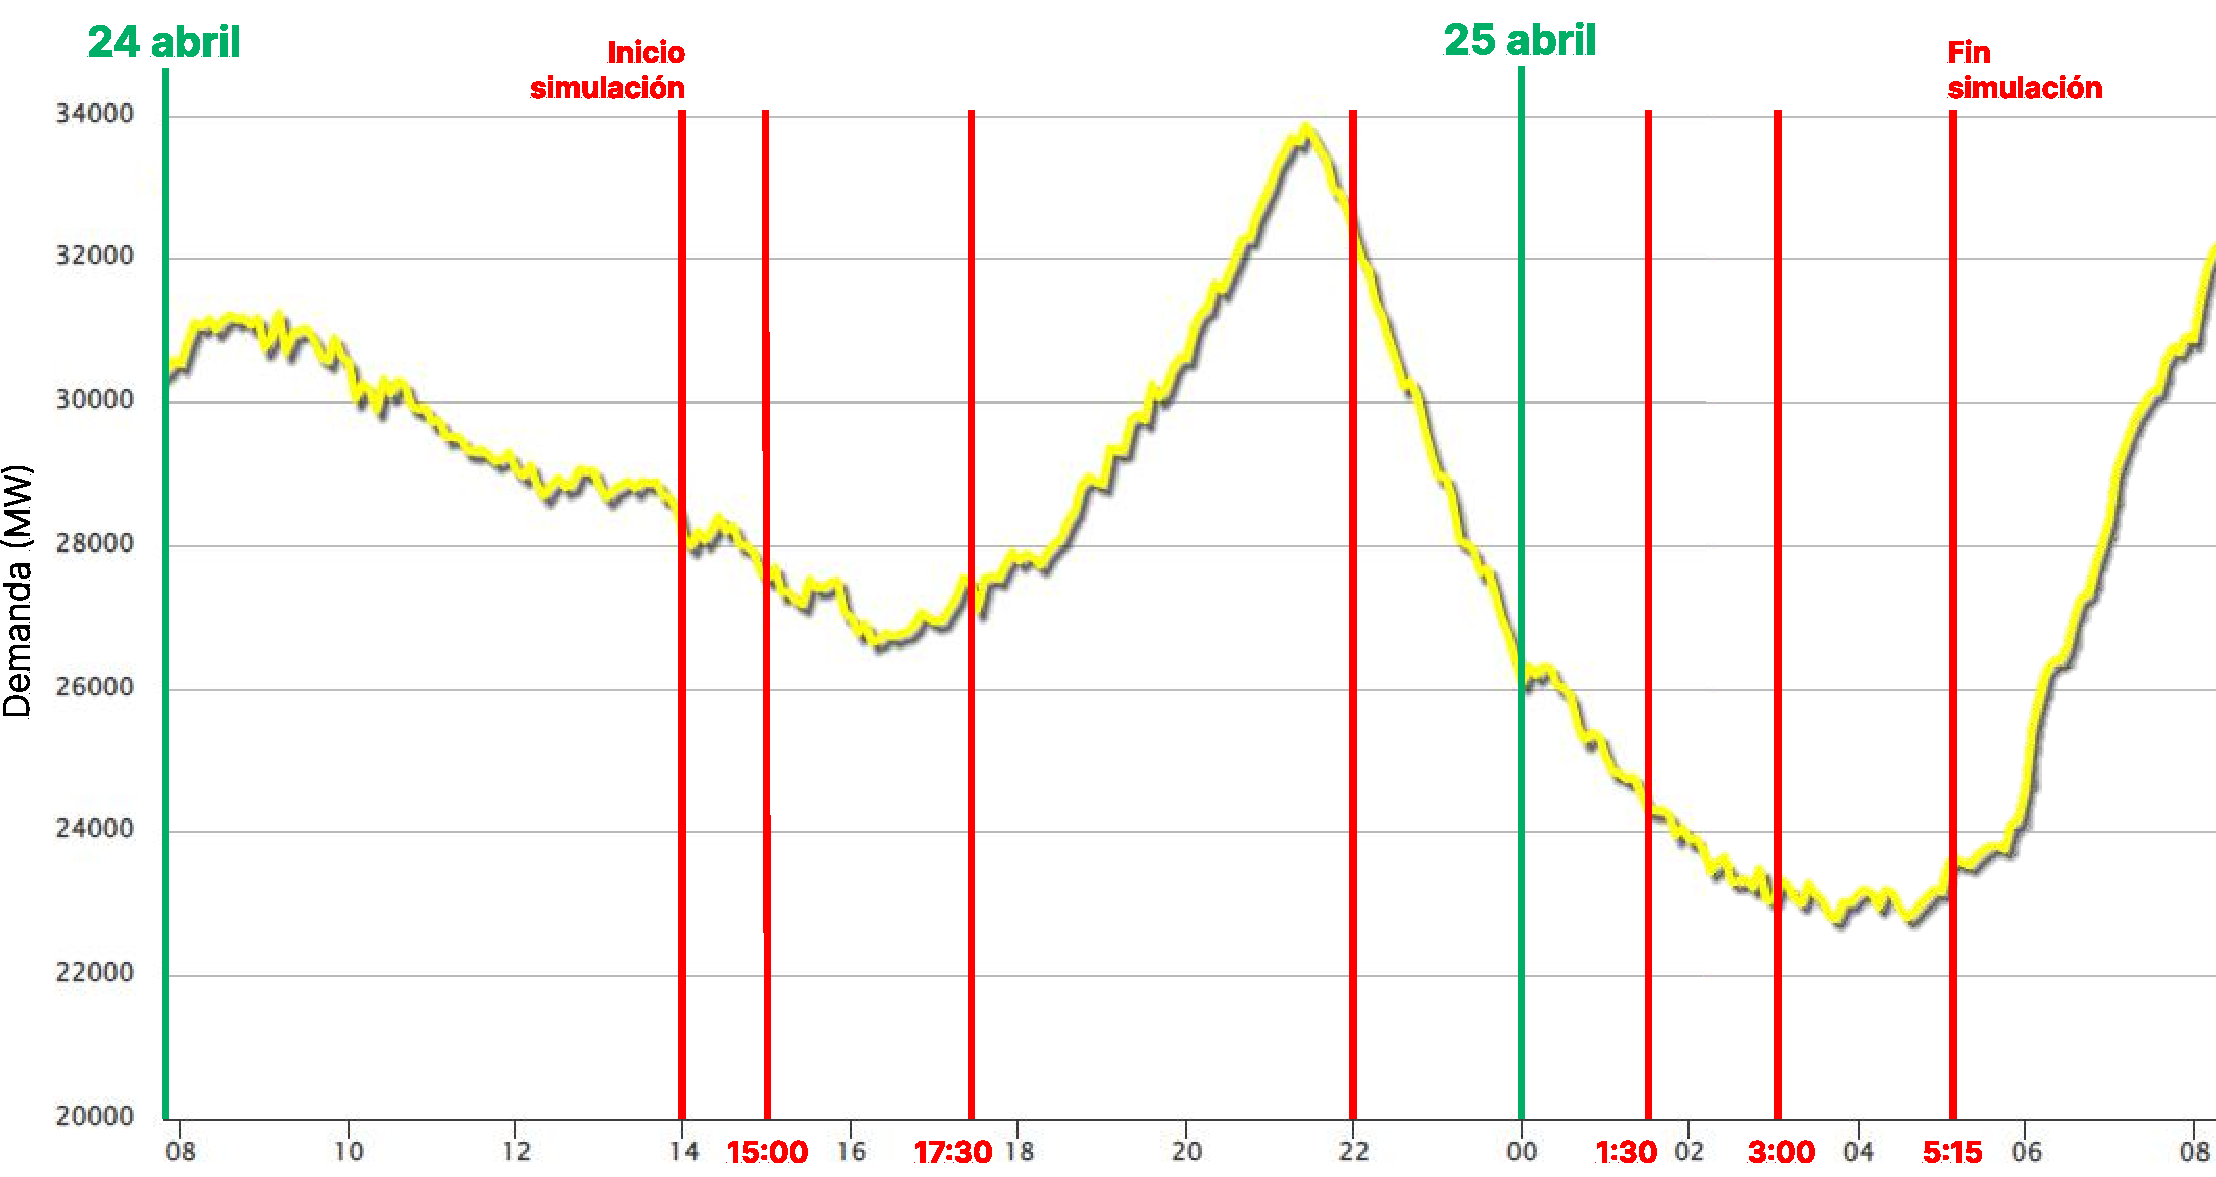
\includegraphics[width=0.9\textwidth]{content/figures/curva_demanda.pdf}
  \caption{Curva de demanda eléctrica en España de los días 24 y 25 de abril de 2024. Se detallan en rojo los momentos importantes de la simulación (\cite{ree_demanda}).}
  \label{fig:curva_demanda}
\end{figure}

\begin{figure}[!h]
  \centering
  \includegraphics[width=\textwidth]{content/figures/sim4_potencias_contextualizacion.pdf}
  \caption{Variaciones de potencia para el seguimiento de la curva de demanda entre los días 24 y 25 de abril de 2024. Se detallan en rojo los momentos importantes de la simulación.}
  \label{fig:sim4_potencias_contextualizacion}
\end{figure}

A continuación, se detallan cronológicamente los cambios en la demanda eléctrica y en la producción renovable que conllevan un consecuente seguimiento de carga:

\begin{itemize}
  \item \underline{14.00 - 15.00 del 24 de abril:} La demanda de energía eléctrica es elevada pero va disminuyendo progresivamente. Se mantiene la central a potencia nominal.
  \item \underline{15.00 - 17.30:} Son unas horas valle en las que la demanda disminuye considerablemente. Se baja la potencia de la planta al 50\% y se mantiene esa potencia durante 2 horas y media:
  \begin{itemize}
    \item \textbf{Variación de potencia:} 46\%
    \item \textbf{Tiempo empleado:} 15 minutos
    \item \textbf{Tasa de variación de potencia:} 3,07\%/min
  \end{itemize} 
  \item \underline{17.30 - 22.00:} A partir de las 17.30 la demanda eléctrica aumenta muy considerablemente, por lo que es necesario volver a generar el 100\% de la potencia:
  \begin{itemize}
    \item \textbf{Variación de potencia:} 46\%
    \item \textbf{Tiempo empleado:} 10 minutos
    \item \textbf{Tasa de variación de potencia:} 4,6\%/min
  \end{itemize} 
  Seguidamente, se mantiene la central a potencia nominal hasta que la curva de demanda comienza a caer muy rápidamente poco antes de las 22.00 de la noche, comenzando el gran valle típico en la curva de demanda eléctrica nocturna. Por tanto, bajamos entorno al 18\% de potencia la las 22.00:
  \begin{itemize}
    \item \textbf{Variación de potencia:} 78\%
    \item \textbf{Tiempo empleado:} 55 minutos
    \item \textbf{Tasa de variación de potencia:} 3,12\%/min
  \end{itemize}
  \item \underline{22.25 - 1.30 del 25 de abril:} La potencia se mantiene entorno al 18\%.
  \item \underline{1.30 - 3.00:} Hasta el momento, toda la maniobra de seguimiento de carga se ha realizado teniendo las fuentes de energía renovable produciendo al máximo ---como es lógico, la solar ha dejado de producir por la noche---. Sin embargo, a partir de la 1.30, se produce una gran calma de viento en la península y la mayoría de aerogeneradores dejan de funcionar. Es necesario, por tanto, aumentar la potencia nuclear, aunque no hasta el 100\%, pues la demanda eléctrica sigue siendo muy baja. Se sube por tanto la potencia entorno al 66\%: 
  \begin{itemize}
    \item \textbf{Variación de potencia:} 48\%
    \item \textbf{Tiempo empleado:} 13 minutos
    \item \textbf{Tasa de variación de potencia:} 3,7\%/min
  \end{itemize}
  Tras mantenerse a ese nivel de potencia durante aproximadamente 1 hora y 15 minutos, la velocidad del viento vuelve a sus valores iniciales y la eólica vuelve a producir prácticamente al máximo. Entonces, se hace necesario disminuir la potencia de la central entorno al 22\%:
  \begin{itemize}
    \item \textbf{Variación de potencia:} 44\%
    \item \textbf{Tiempo empleado:} 12 minutos
    \item \textbf{Tasa de variación de potencia:} 3,67\%/min
  \end{itemize}
  \item \underline{1.30 - 3.00:} Por último, se mantiene el bajo nivel de potencia hasta que se finaliza la simulación a las 5.15  de la madrugada. Si esta siguiera avanzando, a partir de las 6.00 se debería volver a subir a potencia nominal.
\end{itemize}

En definitiva, se ha podido realizar con éxito y rapidez un seguimiento de la curva de demanda eléctrica nacional y de las variaciones en la producción renovable.

\paragraph{Resto de gráficas}

El objetivo fundamental de esta última simulación ha sido ---como se ha explicado anteriormente--- realizar un conjunto de maniobras completo de seguimiento de carga. Por tanto, la gráfica de mayor interés es la de la figura \ref{fig:sim4_potencias_contextualizacion}, en la cual se muestra el seguimiento de carga realizado. Aun así, se han generado el resto de gráficas de las variables más interesantes del reactor para que se pueda observar su comportamiento durante la maniobra. Una apreciación que se muestra muy claramente en estas gráficas es la que ya se ha comentado varias veces anteriormente: cuando el reactor trabaja a potencia nominal o potencias intermedias (50\% o 66\%, en este caso), el comportamiento del sistema es muy estable, mientras que a bajas potencias (18\% o 22\%, en este caso), el sistema presenta las oscilaciones propias de la inestabilidad a potencias bajas.

\begin{figure}[!h]
  \centering
  \includegraphics[width=0.9\textwidth]{content/figures/sim4_temperaturas.pdf}
  \vspace{-0.1cm}
  \caption{Variaciones de temperatura.}
  \label{fig:sim4_temperaturas}
\end{figure}

\begin{figure}[!h]
  \vspace{-0.2cm}
  \centering
  \includegraphics[width=0.9\textwidth]{content/figures/sim4_barras_control.pdf}
  \vspace{-0.1cm}
  \caption{Nivel de extracción de las barras de control.}
  \label{fig:sim4_barras_control}
\end{figure}

\begin{figure}[!h]
  \vspace{-0.2cm}
  \centering
  \includegraphics[width=0.9\textwidth]{content/figures/sim4_boro.pdf}
  \vspace{-0.1cm}
  \caption{Concentración de boro en el circuito primario.}
  \label{fig:sim4_boro}
\end{figure}

\begin{figure}[!h]
  \includegraphics[width=0.5\linewidth]{content/figures/sim4_valvulas_control.pdf} 
  \includegraphics[width=0.5\linewidth]{content/figures/sim4_vapor.pdf}
  \caption{Posición de las válvulas de admisión de vapor (a la izquierda) y caudal de vapor que entra a la turbina (a la derecha).}
  \label{fig:sim4_valvulas_vapor}
\end{figure}

\begin{figure}[!h]
  \centering
  \includegraphics[width=\textwidth]{content/figures/sim4_gen_vapor_camara_imp.pdf}
  \caption{Propiedades del generador de vapor y de la cámara de impulsos.}
  \label{fig:sim4_gen_vapor_camara_imp}
\end{figure}

\begin{figure}[!h]
  \centering
  \includegraphics[width=\textwidth]{content/figures/sim4_presionador.pdf}
  \caption{Propiedades del presionador.}
  \label{fig:sim4_presionador}
\end{figure}
\newpage

% Formato APA (el recomendado para TFG)

\appto{\bibsetup}{\sloppy}

\printbibliography[heading=bibintoc, title=BIBLIOGRAFÍA] % Aparecen únicamente las referencias citadas a lo largo del documento
%%%%%%%%%%%%%%%%%%% - ANEXOS - %%%%%%%%%%%%%%%%%%%

\newpage
\section*{ANEXOS} \label{sec:anexos} % Se añade un asterisco a \section para que el título no esté numerado.
\phantomsection
\addcontentsline{toc}{section}{ANEXOS} % Al utilizar \section* se ha de añadir manualmente el apartado al índice (Table Of Contents, TOC).
\markright{ANEXOS} % Al utilizar \section* se ha de añadir manualmente el título del apartado al encabezado.

\renewcommand{\thesubsection}{\Alph{subsection}} % Se numeran los anexos con letras del alfabeto en lugar de números.
% Se indica que las tablas, figuras y códigos se numeran con el código del anexo (A, B, C, ...) seguido del número de tabla, figura o código dentro del anexo (tabla A.2, figura C.1, etc.)
\renewcommand{\thetable}{\Alph{subsection}.\arabic{table}}
\renewcommand{\thefigure}{\Alph{subsection}.\arabic{figure}}
\renewcommand{\thecode}{\Alph{subsection}.\arabic{code}}

% ---------------- Primer anexo ---------------- %
\setcounter{subsection}{0}
\setcounter{table}{0}
\setcounter{figure}{0}

\subsection{Código} \label{sec:codigo}

Todas las gráficas de las simulaciones realizadas en el \acrshort{sgiz} han sido elaboradas con \textit{Python} a partir de los datos generados en \textit{Excel} por el propio simulador. A continuación, se muestra, a modo de ejemplo, el código para la obtención de una de las gráficas:

\vspace{-5pt}

\begin{code}[H]
\begin{lstlisting}[firstnumber=1, breakindent=55pt]
  # Importación de las librerías necesarias
  import matplotlib.pyplot as plt
  import numpy as np
  import pandas as pd

  # Obtención de datos:
  gen_vapor_camara_imp=pd.read_excel("simulacion3.xlsx","gen_vapor_camara_imp")
  df_gen_vapor_camara_imp=pd.DataFrame=gen_vapor_camara_imp

  tiempo=[]
  for i in range(0,len(df_gen_vapor_camara_imp.tiempo)):
      tiempo.append(df_gen_vapor_camara_imp.tiempo[i].strftime('%H:%M:%S'))
    
  pres_cam_imp=[]
  for i in range(0,len(df_gen_vapor_camara_imp.pres_cam_imp)):
      pres_cam_imp.append(df_gen_vapor_camara_imp.pres_cam_imp[i])

  presion_gen_vapor=[]
  for i in range(0,len(df_gen_vapor_camara_imp.               presion_gen_vapor)):
      presion_gen_vapor.append(df_gen_vapor_camara_imp.presion_gen_vapor[i])

  nivel_gen_vapor=[]
  for i in range(0,len(df_gen_vapor_camara_imp.nivel_gen_vapor)):
      nivel_gen_vapor.append(df_gen_vapor_camara_imp.nivel_gen_vapor[i])

  # Creación del gráfico
  plt.plot(tiempo, presion_camara_impulsos, label='Presión de la cámara de impulsos $(kg/cm^2)$', color='lightcoral')
  plt.plot(tiempo, presion_gen_vapor, label='Presión del generador de vapor $(kg/cm^2)$', color='sandybrown')
  plt.plot(tiempo, nivel_gen_vapor, label='Nivel del generador de vapor R.E. $(cm)$', color='mediumseagreen')

  # Creación de la leyenda y el título
  plt.legend(loc='best')
  plt.xlabel('Tiempo (hh:mm:ss)', family='Times New Roman', size=12)
  plt.title('COMPORTAMIENTO GENERADOR DE VAPOR Y CÁMARA DE IMPULSOS', fontname='Times New Roman', size=18, weight='bold')
  plt.grid(True, color='lightgrey')
  plt.yticks(np.arange(-10,50,5))
  plt.xlim([0, len(tiempo)])
  plt.xticks(np.arange(0,len(tiempo),360))
  plt.xticks(rotation = 10)

  # Mostrar el gráfico
  plt.show()
\end{lstlisting}
\vspace{-5pt}
\caption{Ejemplo del código utilizado para generar las gráficas de las simulaciones. Este en concreto corresponde al código de la figura xx.}
\label{cod:codigo_graficas}
\end{code}

%%%%%%%%%%%%%% - ÍNDICE DE TABLAS - %%%%%%%%%%%%%%
\newpage
\renewcommand{\listtablename}{ÍNDICE DE TABLAS} % Se define el nombre del índice de tablas.
\listoftables % Se genera automáticamente el índice con las distintas tablas del documento (entorno \table o \longtable).
\addcontentsline{toc}{section}{ÍNDICE DE TABLAS} % Se añade manualmente el apartado al índice (Table Of Contents, TOC).


%%%%%%%%%%%%% - ÍNDICE DE FIGURAS - %%%%%%%%%%%%%%
\newpage
\renewcommand{\listfigurename}{ÍNDICE DE FIGURAS} % Se define el nombre del índice de figuras.
\listoffigures % Se genera automáticamente el índice con las distintas figuras del documento (entorno \figure).
\addcontentsline{toc}{section}{ÍNDICE DE FIGURAS} % Se añade manualmente el apartado al índice (Table Of Contents, TOC).

%%%%%%%%%%%%% - ABREVIATURAS, UNIDADES Y ACRÓNIMOS - %%%%%%%%%%%%%%
\newpage
\printnoidxglossary[title={ABREVIATURAS, UNIDADES Y ACRÓNIMOS}] %Si no pongo este comando, no aparece el glosario

%%%%%%%%%%%%% - EJEMPLOS DE FUNCIONALIDADES DE LaTeX  - %%%%%%%%%%%%%%
\input{content/sections/ejemplos_plantilla.tex}


\end{document}